\documentclass[11pt,]{article}
\usepackage[]{mathpazo}
\usepackage{amssymb,amsmath}
\usepackage{ifxetex,ifluatex}
\usepackage{fixltx2e} % provides \textsubscript
\ifnum 0\ifxetex 1\fi\ifluatex 1\fi=0 % if pdftex
  \usepackage[T1]{fontenc}
  \usepackage[utf8]{inputenc}
\else % if luatex or xelatex
  \ifxetex
    \usepackage{mathspec}
  \else
    \usepackage{fontspec}
  \fi
  \defaultfontfeatures{Ligatures=TeX,Scale=MatchLowercase}
\fi
% use upquote if available, for straight quotes in verbatim environments
\IfFileExists{upquote.sty}{\usepackage{upquote}}{}
% use microtype if available
\IfFileExists{microtype.sty}{%
\usepackage{microtype}
\UseMicrotypeSet[protrusion]{basicmath} % disable protrusion for tt fonts
}{}
\usepackage{hyperref}
\PassOptionsToPackage{usenames,dvipsnames}{color} % color is loaded by hyperref
\hypersetup{unicode=true,
            pdftitle={Partner fidelity and asymmetric specialization in ecological networks},
            colorlinks=true,
            linkcolor=black,
            citecolor=black,
            urlcolor=black,
            breaklinks=true}
\urlstyle{same}  % don't use monospace font for urls
\usepackage{natbib}
\bibliographystyle{amnat}
\usepackage{color}
\usepackage{fancyvrb}
\newcommand{\VerbBar}{|}
\newcommand{\VERB}{\Verb[commandchars=\\\{\}]}
\DefineVerbatimEnvironment{Highlighting}{Verbatim}{commandchars=\\\{\}}
% Add ',fontsize=\small' for more characters per line
\newenvironment{Shaded}{}{}
\newcommand{\KeywordTok}[1]{\textcolor[rgb]{0.00,0.00,1.00}{#1}}
\newcommand{\DataTypeTok}[1]{#1}
\newcommand{\DecValTok}[1]{#1}
\newcommand{\BaseNTok}[1]{#1}
\newcommand{\FloatTok}[1]{#1}
\newcommand{\ConstantTok}[1]{#1}
\newcommand{\CharTok}[1]{\textcolor[rgb]{0.00,0.50,0.50}{#1}}
\newcommand{\SpecialCharTok}[1]{\textcolor[rgb]{0.00,0.50,0.50}{#1}}
\newcommand{\StringTok}[1]{\textcolor[rgb]{0.00,0.50,0.50}{#1}}
\newcommand{\VerbatimStringTok}[1]{\textcolor[rgb]{0.00,0.50,0.50}{#1}}
\newcommand{\SpecialStringTok}[1]{\textcolor[rgb]{0.00,0.50,0.50}{#1}}
\newcommand{\ImportTok}[1]{#1}
\newcommand{\CommentTok}[1]{\textcolor[rgb]{0.00,0.50,0.00}{#1}}
\newcommand{\DocumentationTok}[1]{\textcolor[rgb]{0.00,0.50,0.00}{#1}}
\newcommand{\AnnotationTok}[1]{\textcolor[rgb]{0.00,0.50,0.00}{#1}}
\newcommand{\CommentVarTok}[1]{\textcolor[rgb]{0.00,0.50,0.00}{#1}}
\newcommand{\OtherTok}[1]{\textcolor[rgb]{1.00,0.25,0.00}{#1}}
\newcommand{\FunctionTok}[1]{#1}
\newcommand{\VariableTok}[1]{#1}
\newcommand{\ControlFlowTok}[1]{\textcolor[rgb]{0.00,0.00,1.00}{#1}}
\newcommand{\OperatorTok}[1]{#1}
\newcommand{\BuiltInTok}[1]{#1}
\newcommand{\ExtensionTok}[1]{#1}
\newcommand{\PreprocessorTok}[1]{\textcolor[rgb]{1.00,0.25,0.00}{#1}}
\newcommand{\AttributeTok}[1]{#1}
\newcommand{\RegionMarkerTok}[1]{#1}
\newcommand{\InformationTok}[1]{\textcolor[rgb]{0.00,0.50,0.00}{#1}}
\newcommand{\WarningTok}[1]{\textcolor[rgb]{0.00,0.50,0.00}{\textbf{#1}}}
\newcommand{\AlertTok}[1]{\textcolor[rgb]{1.00,0.00,0.00}{#1}}
\newcommand{\ErrorTok}[1]{\textcolor[rgb]{1.00,0.00,0.00}{\textbf{#1}}}
\newcommand{\NormalTok}[1]{#1}
\usepackage{graphicx,grffile}
\makeatletter
\def\maxwidth{\ifdim\Gin@nat@width>\linewidth\linewidth\else\Gin@nat@width\fi}
\def\maxheight{\ifdim\Gin@nat@height>\textheight\textheight\else\Gin@nat@height\fi}
\makeatother
% Scale images if necessary, so that they will not overflow the page
% margins by default, and it is still possible to overwrite the defaults
% using explicit options in \includegraphics[width, height, ...]{}
\setkeys{Gin}{width=\maxwidth,height=\maxheight,keepaspectratio}
\IfFileExists{parskip.sty}{%
\usepackage{parskip}
}{% else
\setlength{\parindent}{0pt}
\setlength{\parskip}{6pt plus 2pt minus 1pt}
}
\setlength{\emergencystretch}{3em}  % prevent overfull lines
\providecommand{\tightlist}{%
  \setlength{\itemsep}{0pt}\setlength{\parskip}{0pt}}
\setcounter{secnumdepth}{0}
% Redefines (sub)paragraphs to behave more like sections
\ifx\paragraph\undefined\else
\let\oldparagraph\paragraph
\renewcommand{\paragraph}[1]{\oldparagraph{#1}\mbox{}}
\fi
\ifx\subparagraph\undefined\else
\let\oldsubparagraph\subparagraph
\renewcommand{\subparagraph}[1]{\oldsubparagraph{#1}\mbox{}}
\fi

%%% Use protect on footnotes to avoid problems with footnotes in titles
\let\rmarkdownfootnote\footnote%
\def\footnote{\protect\rmarkdownfootnote}

%%% Change title format to be more compact
\usepackage{titling}

% Create subtitle command for use in maketitle
\providecommand{\subtitle}[1]{
  \posttitle{
    \begin{center}\large#1\end{center}
    }
}

\setlength{\droptitle}{-2em}

  \title{Partner fidelity and asymmetric specialization in ecological networks}
    \pretitle{\vspace{\droptitle}\centering\huge}
  \posttitle{\par}
  \subtitle{Supplementary material}
  \author{}
    \preauthor{}\postauthor{}
    \date{}
    \predate{}\postdate{}
  
%%% Modified from Latex Template for Am. Nat., many other details aren't necessary because they are specified in YAML header of Rmarkdown document.
\usepackage{fullpage}
\linespread{1.7}
\usepackage{lineno}

% code below is important for holding figure positions in main text. Make sure to set fig.pos="H" in code chunk for figure.
\usepackage{float}
\let\origfigure\figure
\let\endorigfigure\endfigure
\renewenvironment{figure}[1][2] {
    \expandafter\origfigure\expandafter[H]
} {
    \endorigfigure
}
\usepackage{booktabs}
\usepackage{longtable}
\usepackage{array}
\usepackage{multirow}
\usepackage{wrapfig}
\usepackage{float}
\usepackage{colortbl}
\usepackage{pdflscape}
\usepackage{tabu}
\usepackage{threeparttable}
\usepackage{threeparttablex}
\usepackage[normalem]{ulem}
\usepackage{makecell}
\usepackage{xcolor}

\begin{document}
\maketitle

{
\hypersetup{linkcolor=black}
\setcounter{tocdepth}{2}
\tableofcontents
}
\newpage

All data and code to reproduce the analyses presented below are
available on GitHub
(\url{https://github.com/mabarbour/partner_fidelity}) and have been
archived on Zenodo (\url{https://doi.org/10.5281/zenodo.3246344}).

\subsection{Dataset}\label{dataset}

Here's a summary of the full dataset we used in our analyses (table
\ref{tab:full-dataset}).

\begin{table}[!h]

\caption{\label{tab:full-dataset}Random sample of 10 rows from the full dataset.}
\centering
\resizebox{\linewidth}{!}{
\begin{tabular}{rllrrllll}
\toprule
connected & type & subtype & r\_ND & c\_ND & resource\_sp & consumer\_sp & id\_pair & network\_id\\
\midrule
0 & A & HostParasite & 0.35 & 0.07 & Cricetulus migratorius & Frontopsylla protera & 3206 & A\_HP\_029\\
0 & A & HostParasite & 0.47 & 0.25 & Alticola argentatus & Frontopsylla elata & 2710 & A\_HP\_011\\
0 & M & PlantPollinator & 0.02 & 0.11 & Hieracium pilosella & Formica fusca & 839 & M\_PL\_047\\
1 & A & HostParasite & 0.86 & 0.58 & Microtus arvalis & Megabothris turbidus & 3486 & A\_HP\_048\\
1 & A & PlantHerbivore & 0.25 & 0.43 & Xanthocephalum texanum & Melanoplus desultorius & 2201 & A\_PH\_005\\
\addlinespace
1 & A & PlantHerbivore & 0.42 & 0.19 & Croton pottsii & Melanoplus gladstoni & 2159 & A\_PH\_005\\
1 & M & PlantPollinator & 0.05 & 0.06 & Ranunculus japonicus & Melanostoma scalare & 1434 & M\_PL\_053\\
1 & M & PlantPollinator & 0.16 & 0.05 & Tanacetum vulgare & Sphaerophoria scripta & 1824 & M\_PL\_018\\
1 & A & HostParasite & 0.71 & 0.13 & Clethrionomys glareolus & Rhadinopsylla integella & 3008 & A\_HP\_018\\
0 & M & PlantPollinator & 0.02 & 0.59 & Cirsium arvense & Bombus pascuorum & 331 & M\_PL\_006\\
\bottomrule
\end{tabular}}
\end{table}

\begin{itemize}
\tightlist
\item
  \textbf{connected}: observed species interaction (0 = no interaction
  observed, 1 = interaction observed)
\item
  \textbf{type}: type of interaction (A = antagonistic; M = mutualistic)
\item
  \textbf{subtype}: specific type of interaction (PlantPollinator,
  PlantHerbivore, PlantSeedDisperser, HostParasite)
\item
  \textbf{r\_ND}: normalized degree of resource species (mean = 0.28, SD
  = 0.24)
\item
  \textbf{c\_ND}: normalized degree of consumer species (mean = 0.28, SD
  = 0.23)
\item
  \textbf{resource\_sp}: resource species ID (n = 444)
\item
  \textbf{consumer\_sp}: consumer species ID (n = 803)
\item
  \textbf{id\_pair}: consumer-resource interaction ID (n = 4075)
\item
  \textbf{network\_id}: ecological network ID (n = 133; labels match
  those on the \href{http://www.web-of-life.es/}{Web of Life})
\end{itemize}

We also analyze a subset of this data that only consists of weighted
networks (table \ref{tab:weighted-subset-dataset}), which we use to
investigate the effects of sampling effort.

\begin{table}[!h]

\caption{\label{tab:weighted-subset-dataset}Random sample of 10 rows from the subset of weighted networks.}
\centering
\resizebox{\linewidth}{!}{
\begin{tabular}{rllrrrrllll}
\toprule
connected & type & subtype & r\_ND & c\_ND & log.sum\_r & log.sum\_c & resource\_sp & consumer\_sp & id\_pair & network\_id\\
\midrule
0 & M & PlantPollinator & 0.01 & 0.02 & 2.40 & 1.95 & Reynoutria japonica & Eristalis tenax & 1570 & M\_PL\_044\\
0 & A & HostParasite & 0.16 & 0.40 & 2.40 & 4.91 & Apodemus peninsulae & Ctenophthalmus congeneroides & 2793 & A\_HP\_049\\
1 & A & HostParasite & 0.47 & 0.69 & 4.66 & 6.93 & Apodemus uralensis & Corrodopsylla birulai & 2837 & A\_HP\_020\\
0 & M & PlantSeedDisperser & 0.23 & 0.08 & 1.39 & 1.39 & Cecropia schreberiana & Tyrannus dominicensis & 2441 & M\_SD\_005\\
0 & A & HostParasite & 0.54 & 0.15 & 5.98 & 2.77 & Microtus arvalis & Neopsylla pleskei & 3510 & A\_HP\_044\\
\addlinespace
0 & M & PlantPollinator & 0.06 & 0.09 & 3.87 & 2.83 & Deutzia crenata & Episyrphus balteatus & 561 & M\_PL\_054\\
0 & M & PlantSeedDisperser & 0.15 & 0.44 & 2.56 & 4.14 & Miconia affinis & Loxigilla portoricensis & 2569 & M\_SD\_004\\
1 & A & HostParasite & 0.65 & 0.56 & 7.30 & 4.63 & Clethrionomys rutilus & Frontopsylla elata & 3048 & A\_HP\_020\\
1 & A & HostParasite & 0.12 & 1.00 & 2.56 & 5.24 & Cricetus cricetus & Rhadinopsylla li & 3358 & A\_HP\_044\\
0 & A & HostParasite & 0.43 & 0.06 & 7.94 & 0.69 & Cricetulus migratorius & Rhadinopsylla ucrainica & 3249 & A\_HP\_006\\
\bottomrule
\end{tabular}}
\end{table}

\begin{itemize}
\tightlist
\item
  \textbf{connected}: 0 = no interaction observed, 1 = interaction
  observed
\item
  \textbf{type}: A = antagonistic, M = mutualistic
\item
  \textbf{subtype}: HostParasite, PlantPollinator, PlantSeedDisperser
\item
  \textbf{r\_ND}: mean = 0.35, SD = 0.2
\item
  \textbf{c\_ND}: mean = 0.34, SD = 0.2
\item
  \textbf{log.sum\_r}: mean = 4.5, SD = 2.2
\item
  \textbf{log.sum\_c}: mean = 4, SD = 2.1
\item
  \textbf{resource\_sp}: n = 167
\item
  \textbf{consumer\_sp}: n = 291
\item
  \textbf{id\_pair}: n = 1813
\item
  \textbf{network\_id}: n = 68
\end{itemize}

Note that the general structure of the subset of data is the same as the
full dataset, except we have added two new variables. These variables
correspond to the logarithm of observed interactions (sum of interaction
frequency) for a resource (\textbf{log.sum\_r}) and consumer
(\textbf{log.sum\_c}) in a network. These variables give information on
sampling effort. Note also that we only have three interaction
\textbf{subtype}s now (no weighted networks for PlantHerbivore).

Prior to our analyses, we scaled normalized degree (mean = 0, SD = 1)
for both consumers and resources. This allowed us to interpret both main
effects and statistical interactions within the same model, and also
allowed us to easily compare their effect sizes \citep{Schielzeth2010}.
We also scaled the logarithm of observed interactions for both consumers
and resources.

\begin{Shaded}
\begin{Highlighting}[]
\NormalTok{full.df <-}\StringTok{ }\NormalTok{full.df }\OperatorTok
\StringTok{  }\KeywordTok{mutate}\NormalTok{(}\DataTypeTok{sc.r_ND =} \KeywordTok{scale}\NormalTok{(r_ND),}
         \DataTypeTok{sc.c_ND =} \KeywordTok{scale}\NormalTok{(c_ND))}

\NormalTok{weighted_subset.df <-}\StringTok{ }\NormalTok{weighted_subset.df }\OperatorTok
\StringTok{  }\KeywordTok{mutate}\NormalTok{(}\DataTypeTok{sc.r_ND =} \KeywordTok{scale}\NormalTok{(r_ND),}
         \DataTypeTok{sc.c_ND =} \KeywordTok{scale}\NormalTok{(c_ND),}
         \DataTypeTok{sc.log.sum_r =} \KeywordTok{scale}\NormalTok{(log.sum_r),}
         \DataTypeTok{sc.log.sum_c =} \KeywordTok{scale}\NormalTok{(log.sum_c))}
\end{Highlighting}
\end{Shaded}

For \textbf{type}, we created a contrast so that the intercept term
represents the average probability (Ave) of an interaction across
mutualistic (M) and antagonistic (A) interactions, and this coefficient
represents the effect of mutualistic (relative to antagonistic)
interactions (table \ref{tab:type-contrasts}).

\begin{table}[!h]

\caption{\label{tab:type-contrasts}Contrasts for \textbf{type}.}
\centering
\begin{tabular}{lrr}
\toprule
  & A & M\\
\midrule
Ave & 0.5 & 0.5\\
\_M.vs.A & -1.0 & 1.0\\
\bottomrule
\end{tabular}
\end{table}

To test for the effect of network \textbf{subtype} within each
\textbf{type}, we create two new variables:

\begin{Shaded}
\begin{Highlighting}[]
\NormalTok{full.df <-}\StringTok{ }\NormalTok{full.df }\OperatorTok
\StringTok{  }\KeywordTok{mutate}\NormalTok{(}\DataTypeTok{subtype_Herb.vs.Para =} \KeywordTok{ifelse}\NormalTok{(type }\OperatorTok{==}\StringTok{ "M"}\NormalTok{, }\DecValTok{0}\NormalTok{,}
                            \KeywordTok{ifelse}\NormalTok{(subtype }\OperatorTok{==}\StringTok{ "PlantHerbivore"}\NormalTok{, }\DecValTok{1}\OperatorTok{/}\DecValTok{2}\NormalTok{, }\OperatorTok{-}\DecValTok{1}\OperatorTok{/}\DecValTok{2}\NormalTok{)),}
         \DataTypeTok{subtype_Poll.vs.Disp =} \KeywordTok{ifelse}\NormalTok{(type }\OperatorTok{==}\StringTok{ "A"}\NormalTok{, }\DecValTok{0}\NormalTok{,}
                            \KeywordTok{ifelse}\NormalTok{(subtype }\OperatorTok{==}\StringTok{ "PlantPollinator"}\NormalTok{, }\DecValTok{1}\OperatorTok{/}\DecValTok{2}\NormalTok{, }\OperatorTok{-}\DecValTok{1}\OperatorTok{/}\DecValTok{2}\NormalTok{)))}
\end{Highlighting}
\end{Shaded}

Now, \textbf{subtype\_Herb.vs.Para} tests for an effect of herbivory
(relative to parasitism), and \textbf{subtype\_Poll.vs.Disp} tests for
an effect of pollination (relative to seed dispersal).

Since we do not have multiple \textbf{subtype}s for antagonistic
interactions in the data subset, we only fit a \textbf{subtype} contrast
for mutualistic interactions.

\begin{Shaded}
\begin{Highlighting}[]
\NormalTok{weighted_subset.df <-}\StringTok{ }\NormalTok{weighted_subset.df }\OperatorTok
\StringTok{  }\KeywordTok{mutate}\NormalTok{(}\DataTypeTok{subtype_Poll.vs.Disp =} \KeywordTok{ifelse}\NormalTok{(type }\OperatorTok{==}\StringTok{ "A"}\NormalTok{, }\DecValTok{0}\NormalTok{,}
                            \KeywordTok{ifelse}\NormalTok{(subtype }\OperatorTok{==}\StringTok{ "PlantPollinator"}\NormalTok{, }\DecValTok{1}\OperatorTok{/}\DecValTok{2}\NormalTok{, }\OperatorTok{-}\DecValTok{1}\OperatorTok{/}\DecValTok{2}\NormalTok{)))}
\end{Highlighting}
\end{Shaded}

~

\subsection{Statistical Models}\label{statistical-models}

We fit the following statistical model to our full dataset:

\begin{Shaded}
\begin{Highlighting}[]
\NormalTok{interaction.formula <-}\StringTok{ }\KeywordTok{brmsformula}\NormalTok{(}
\NormalTok{  connected }\OperatorTok{~}\StringTok{ }\NormalTok{type }\OperatorTok{+}\StringTok{ }\NormalTok{subtype_Herb.vs.Para }\OperatorTok{+}\StringTok{ }\NormalTok{subtype_Poll.vs.Disp }\OperatorTok{+}\StringTok{ }\NormalTok{sc.r_ND }\OperatorTok{+}\StringTok{ }\NormalTok{sc.c_ND }\OperatorTok{+}\StringTok{ }
\StringTok{    }\NormalTok{type}\OperatorTok{:}\NormalTok{sc.r_ND }\OperatorTok{+}\StringTok{ }\NormalTok{type}\OperatorTok{:}\NormalTok{sc.c_ND }\OperatorTok{+}\StringTok{ }\NormalTok{sc.r_ND}\OperatorTok{:}\NormalTok{sc.c_ND }\OperatorTok{+}
\StringTok{    }\NormalTok{type}\OperatorTok{:}\NormalTok{sc.r_ND}\OperatorTok{:}\NormalTok{sc.c_ND }\OperatorTok{+}
\StringTok{    }\NormalTok{(}\DecValTok{1} \OperatorTok{|}\StringTok{ }\NormalTok{resource_sp) }\OperatorTok{+}\StringTok{ }\NormalTok{(}\DecValTok{1} \OperatorTok{|}\StringTok{ }\NormalTok{consumer_sp) }\OperatorTok{+}\StringTok{ }\NormalTok{(}\DecValTok{1} \OperatorTok{|}\StringTok{ }\NormalTok{id_pair) }\OperatorTok{+}\StringTok{ }\NormalTok{(}\DecValTok{1} \OperatorTok{|}\StringTok{ }\NormalTok{network_id),}
  \DataTypeTok{family =} \KeywordTok{bernoulli}\NormalTok{(}\DataTypeTok{link =} \StringTok{"logit"}\NormalTok{)}
\NormalTok{)}
\end{Highlighting}
\end{Shaded}

~

and a similar model to the data subset:

\begin{Shaded}
\begin{Highlighting}[]
\NormalTok{interaction_subset.formula <-}\StringTok{ }\KeywordTok{brmsformula}\NormalTok{(}
\NormalTok{  connected }\OperatorTok{~}\StringTok{ }\NormalTok{type }\OperatorTok{+}\StringTok{ }\NormalTok{subtype_Poll.vs.Disp }\OperatorTok{+}\StringTok{ }\NormalTok{sc.r_ND }\OperatorTok{+}\StringTok{ }\NormalTok{sc.c_ND }\OperatorTok{+}\StringTok{ }
\StringTok{    }\NormalTok{type}\OperatorTok{:}\NormalTok{sc.r_ND }\OperatorTok{+}\StringTok{ }\NormalTok{type}\OperatorTok{:}\NormalTok{sc.c_ND }\OperatorTok{+}\StringTok{ }\NormalTok{sc.r_ND}\OperatorTok{:}\NormalTok{sc.c_ND }\OperatorTok{+}
\StringTok{    }\NormalTok{type}\OperatorTok{:}\NormalTok{sc.r_ND}\OperatorTok{:}\NormalTok{sc.c_ND }\OperatorTok{+}
\StringTok{    }\NormalTok{(}\DecValTok{1} \OperatorTok{|}\StringTok{ }\NormalTok{resource_sp) }\OperatorTok{+}\StringTok{ }\NormalTok{(}\DecValTok{1} \OperatorTok{|}\StringTok{ }\NormalTok{consumer_sp) }\OperatorTok{+}\StringTok{ }\NormalTok{(}\DecValTok{1} \OperatorTok{|}\StringTok{ }\NormalTok{id_pair) }\OperatorTok{+}\StringTok{ }\NormalTok{(}\DecValTok{1} \OperatorTok{|}\StringTok{ }\NormalTok{network_id),}
  \DataTypeTok{family =} \KeywordTok{bernoulli}\NormalTok{(}\DataTypeTok{link =} \StringTok{"logit"}\NormalTok{) }
\NormalTok{) }\CommentTok{# note that we do not include subtype_Herb.vs.Para, since we do not have}
\CommentTok{# PlantHerbivore interactions in the weighted subset.}
\end{Highlighting}
\end{Shaded}

These models analyze the probability of a species interaction as a
function of all main effects, as well as two- and three-way interactions
between the type of interaction (\textbf{type}) and scaled normalized
degree of resources (\textbf{sc.r\_ND}) and consumers
(\textbf{sc.c\_ND})(fixed effects). Note that we only test for main
effects of network subtypes within the type of interaction. This model
also allows the probability of interactions to vary among resource and
consumer species, the unique consumer-resource pair, as well as among
unique ecological networks (random effects). Note that by including the
unique consumer-resource pair as a random effect, we are testing how the
different factors in our model influence partner fidelity (i.e.,
probability of two species to interact when they co-occur). Note also
that specifying a Bernoulli distribution on the logit scale for the
error distribution in our model makes it so that the fixed and random
effects in our statistical model represent effects on the log odds of
partner fidelity.

For the subset of data, we also fit the following model:

\begin{Shaded}
\begin{Highlighting}[]
\NormalTok{sampling_effects.formula <-}\StringTok{ }\KeywordTok{brmsformula}\NormalTok{(}
\NormalTok{  connected }\OperatorTok{~}\StringTok{ }\NormalTok{type }\OperatorTok{+}\StringTok{ }\NormalTok{subtype_Poll.vs.Disp }\OperatorTok{+}\StringTok{ }\NormalTok{sc.log.sum_r }\OperatorTok{+}\StringTok{ }\NormalTok{sc.log.sum_c }\OperatorTok{+}\StringTok{ }
\StringTok{    }\NormalTok{type}\OperatorTok{:}\NormalTok{sc.log.sum_r }\OperatorTok{+}\StringTok{ }\NormalTok{type}\OperatorTok{:}\NormalTok{sc.log.sum_c }\OperatorTok{+}\StringTok{ }\NormalTok{sc.log.sum_r}\OperatorTok{:}\NormalTok{sc.log.sum_c }\OperatorTok{+}
\StringTok{    }\NormalTok{type}\OperatorTok{:}\NormalTok{sc.log.sum_r}\OperatorTok{:}\NormalTok{sc.log.sum_c }\OperatorTok{+}
\StringTok{    }\NormalTok{(}\DecValTok{1} \OperatorTok{|}\StringTok{ }\NormalTok{resource_sp) }\OperatorTok{+}\StringTok{ }\NormalTok{(}\DecValTok{1} \OperatorTok{|}\StringTok{ }\NormalTok{consumer_sp) }\OperatorTok{+}\StringTok{ }\NormalTok{(}\DecValTok{1} \OperatorTok{|}\StringTok{ }\NormalTok{id_pair) }\OperatorTok{+}\StringTok{ }\NormalTok{(}\DecValTok{1} \OperatorTok{|}\StringTok{ }\NormalTok{network_id),}
  \DataTypeTok{family =} \KeywordTok{bernoulli}\NormalTok{(}\DataTypeTok{link =} \StringTok{"logit"}\NormalTok{)}
\NormalTok{) }\CommentTok{# again, we do not include subtype_Herb.vs.Para, since we do not have}
\CommentTok{# PlantHerbivore interactions in the weighted subset.}
\end{Highlighting}
\end{Shaded}

This model is similar to the previous models except that we substitute
the logarithm of observed interactions for the normalized degree. The
logic behind this model is that, if we observe the same patterns as we
do when using normalized degree, then our results could simply be due to
variation in sampling effort.

~

\subsection{Choosing Priors}\label{choosing-priors}

Given the number of random effects in our model, we used a Bayesian
approach to estimate our model's parameters (as advised by
\href{https://www.sciencedirect.com/science/article/pii/S0169534709000196}{Bolker
et al. 2008}). This required us to choose prior distributions for the
fixed and random effects in our model.

We specified the following priors in our models:

\begin{Shaded}
\begin{Highlighting}[]
\NormalTok{interaction.priors <-}\StringTok{ }\KeywordTok{c}\NormalTok{(}
  \KeywordTok{set_prior}\NormalTok{(}\StringTok{"normal(0,2)"}\NormalTok{, }\DataTypeTok{class =} \StringTok{"b"}\NormalTok{, }\DataTypeTok{coef =} \StringTok{"type_M.vs.A"}\NormalTok{),}
  \KeywordTok{set_prior}\NormalTok{(}\StringTok{"normal(0,2)"}\NormalTok{, }\DataTypeTok{class =} \StringTok{"b"}\NormalTok{, }\DataTypeTok{coef =} \StringTok{"subtype_Herb.vs.Para"}\NormalTok{),}
  \KeywordTok{set_prior}\NormalTok{(}\StringTok{"normal(0,2)"}\NormalTok{, }\DataTypeTok{class =} \StringTok{"b"}\NormalTok{, }\DataTypeTok{coef =} \StringTok{"subtype_Poll.vs.Disp"}\NormalTok{),}
  \KeywordTok{set_prior}\NormalTok{(}\StringTok{"normal(1,2)"}\NormalTok{, }\DataTypeTok{class =} \StringTok{"b"}\NormalTok{, }\DataTypeTok{coef =} \StringTok{"sc.r_ND"}\NormalTok{),}
  \KeywordTok{set_prior}\NormalTok{(}\StringTok{"normal(1,2)"}\NormalTok{, }\DataTypeTok{class =} \StringTok{"b"}\NormalTok{, }\DataTypeTok{coef =} \StringTok{"sc.c_ND"}\NormalTok{),}
  \KeywordTok{set_prior}\NormalTok{(}\StringTok{"normal(0,2)"}\NormalTok{, }\DataTypeTok{class =} \StringTok{"b"}\NormalTok{, }\DataTypeTok{coef =} \StringTok{"sc.r_ND:sc.c_ND"}\NormalTok{),}
  \KeywordTok{set_prior}\NormalTok{(}\StringTok{"normal(0,2)"}\NormalTok{, }\DataTypeTok{class =} \StringTok{"b"}\NormalTok{, }\DataTypeTok{coef =} \StringTok{"type_M.vs.A:sc.r_ND"}\NormalTok{),}
  \KeywordTok{set_prior}\NormalTok{(}\StringTok{"normal(0,2)"}\NormalTok{, }\DataTypeTok{class =} \StringTok{"b"}\NormalTok{, }\DataTypeTok{coef =} \StringTok{"type_M.vs.A:sc.c_ND"}\NormalTok{),}
  \KeywordTok{set_prior}\NormalTok{(}\StringTok{"normal(0,2)"}\NormalTok{, }\DataTypeTok{class =} \StringTok{"b"}\NormalTok{, }\DataTypeTok{coef =} \StringTok{"type_M.vs.A:sc.r_ND:sc.c_ND"}\NormalTok{),}
  \KeywordTok{set_prior}\NormalTok{(}\StringTok{"normal(0,2)"}\NormalTok{, }\DataTypeTok{class =} \StringTok{"sd"}\NormalTok{))}

\NormalTok{interaction_subset.priors <-}\StringTok{ }\KeywordTok{c}\NormalTok{(}
  \KeywordTok{set_prior}\NormalTok{(}\StringTok{"normal(0,2)"}\NormalTok{, }\DataTypeTok{class =} \StringTok{"b"}\NormalTok{, }\DataTypeTok{coef =} \StringTok{"type_M.vs.A"}\NormalTok{),}
  \KeywordTok{set_prior}\NormalTok{(}\StringTok{"normal(0,2)"}\NormalTok{, }\DataTypeTok{class =} \StringTok{"b"}\NormalTok{, }\DataTypeTok{coef =} \StringTok{"subtype_Poll.vs.Disp"}\NormalTok{),}
  \KeywordTok{set_prior}\NormalTok{(}\StringTok{"normal(1,2)"}\NormalTok{, }\DataTypeTok{class =} \StringTok{"b"}\NormalTok{, }\DataTypeTok{coef =} \StringTok{"sc.r_ND"}\NormalTok{),}
  \KeywordTok{set_prior}\NormalTok{(}\StringTok{"normal(1,2)"}\NormalTok{, }\DataTypeTok{class =} \StringTok{"b"}\NormalTok{, }\DataTypeTok{coef =} \StringTok{"sc.c_ND"}\NormalTok{),}
  \KeywordTok{set_prior}\NormalTok{(}\StringTok{"normal(0,2)"}\NormalTok{, }\DataTypeTok{class =} \StringTok{"b"}\NormalTok{, }\DataTypeTok{coef =} \StringTok{"sc.r_ND:sc.c_ND"}\NormalTok{),}
  \KeywordTok{set_prior}\NormalTok{(}\StringTok{"normal(0,2)"}\NormalTok{, }\DataTypeTok{class =} \StringTok{"b"}\NormalTok{, }\DataTypeTok{coef =} \StringTok{"type_M.vs.A:sc.r_ND"}\NormalTok{),}
  \KeywordTok{set_prior}\NormalTok{(}\StringTok{"normal(0,2)"}\NormalTok{, }\DataTypeTok{class =} \StringTok{"b"}\NormalTok{, }\DataTypeTok{coef =} \StringTok{"type_M.vs.A:sc.c_ND"}\NormalTok{),}
  \KeywordTok{set_prior}\NormalTok{(}\StringTok{"normal(0,2)"}\NormalTok{, }\DataTypeTok{class =} \StringTok{"b"}\NormalTok{, }\DataTypeTok{coef =} \StringTok{"type_M.vs.A:sc.r_ND:sc.c_ND"}\NormalTok{),}
  \KeywordTok{set_prior}\NormalTok{(}\StringTok{"normal(0,2)"}\NormalTok{, }\DataTypeTok{class =} \StringTok{"sd"}\NormalTok{))}

\NormalTok{sampling_effect.priors <-}\StringTok{ }\KeywordTok{c}\NormalTok{(}
  \KeywordTok{set_prior}\NormalTok{(}\StringTok{"normal(0,2)"}\NormalTok{, }\DataTypeTok{class =} \StringTok{"b"}\NormalTok{, }\DataTypeTok{coef =} \StringTok{"type_M.vs.A"}\NormalTok{),}
  \KeywordTok{set_prior}\NormalTok{(}\StringTok{"normal(0,2)"}\NormalTok{, }\DataTypeTok{class =} \StringTok{"b"}\NormalTok{, }\DataTypeTok{coef =} \StringTok{"subtype_Poll.vs.Disp"}\NormalTok{),}
  \KeywordTok{set_prior}\NormalTok{(}\StringTok{"normal(1,2)"}\NormalTok{, }\DataTypeTok{class =} \StringTok{"b"}\NormalTok{, }\DataTypeTok{coef =} \StringTok{"sc.log.sum_r"}\NormalTok{),}
  \KeywordTok{set_prior}\NormalTok{(}\StringTok{"normal(1,2)"}\NormalTok{, }\DataTypeTok{class =} \StringTok{"b"}\NormalTok{, }\DataTypeTok{coef =} \StringTok{"sc.log.sum_c"}\NormalTok{),}
  \KeywordTok{set_prior}\NormalTok{(}\StringTok{"normal(0,2)"}\NormalTok{, }\DataTypeTok{class =} \StringTok{"b"}\NormalTok{, }\DataTypeTok{coef =} \StringTok{"sc.log.sum_r:sc.log.sum_c"}\NormalTok{),}
  \KeywordTok{set_prior}\NormalTok{(}\StringTok{"normal(0,2)"}\NormalTok{, }\DataTypeTok{class =} \StringTok{"b"}\NormalTok{, }\DataTypeTok{coef =} \StringTok{"type_M.vs.A:sc.log.sum_r"}\NormalTok{),}
  \KeywordTok{set_prior}\NormalTok{(}\StringTok{"normal(0,2)"}\NormalTok{, }\DataTypeTok{class =} \StringTok{"b"}\NormalTok{, }\DataTypeTok{coef =} \StringTok{"type_M.vs.A:sc.log.sum_c"}\NormalTok{),}
  \KeywordTok{set_prior}\NormalTok{(}\StringTok{"normal(0,2)"}\NormalTok{, }\DataTypeTok{class =} \StringTok{"b"}\NormalTok{, }\DataTypeTok{coef =} \StringTok{"type_M.vs.A:sc.log.sum_r:sc.log.sum_c"}\NormalTok{),}
  \KeywordTok{set_prior}\NormalTok{(}\StringTok{"normal(0,2)"}\NormalTok{, }\DataTypeTok{class =} \StringTok{"sd"}\NormalTok{))}
\end{Highlighting}
\end{Shaded}

Choosing priors requires thinking on the scale of the model. Therefore,
we first give a description of what each term quantifies in these models
before justifying our choices. Note that all of these fixed effects
(except for \textbf{Intercept}) can be interpreted as an effect on the
log-odds of partner fidelity:

\begin{itemize}
\tightlist
\item
  \textbf{Intercept} = log-odds of partner fidelity across interaction
  types at the mean normalized degree of resources and consumers.
\item
  \textbf{type\_M.vs.A} = effect of a mutualistic interaction (relative
  to antagonistic).
\item
  \textbf{subtype\_Herb.vs.Para} = effect of herbivory relative to
  parasitism.
\item
  \textbf{subtype\_Poll.vs.Disp} = effect of pollination relative to
  seed disperser.
\item
  \textbf{sc.r\_ND} = effect of 1 SD increase in resource normalized
  degree across interaction types.
\item
  \textbf{sc.c\_ND} = effect of 1 SD increase in consumer normalized
  degree across interaction types.
\item
  \textbf{type\_M.vs.A:sc.r\_ND} = effect of a mutualistic interaction
  (relative to antagonistic) on a 1 SD increase in resource normalized
  degree.
\item
  \textbf{type\_M.vs.A:sc.c\_ND} = effect of a mutualistic interaction
  (relative to antagonistic) on a 1 SD increase in consumer normalized
  degree.
\item
  \textbf{sc.r\_ND:sc.c\_ND} = nonadditive effect of 1 SD increase in
  resource and consumer normalized degree across interaction types. A
  positive value indicates that symmetry in partners normalized degree
  increases partner fidelity, whereas a negative value indicates that
  \emph{asymmetry} in partners normalized degree increases partner
  fidelity (see justification for this in section
  \protect\hyperlink{asymmetry-effect}{\textbf{Asymmetry effect}}).
\item
  \textbf{type\_M.vs.A:sc.r\_ND:sc.c\_ND} = nonadditive effect of a
  mutualistic interaction (relative to antagonistic) on a 1 SD increase
  in resource and consumer normalized degree. A positive value indicates
  that mutualistic interactions enhance the effects of symmetry on
  partner fidelity, whereas a negative value indicates that mutualistic
  interactions enhance the effects of \emph{asymmetry}.
\end{itemize}

For each of our random effects (\textbf{resource\_sp},
\textbf{consumer\_sp}, \textbf{id\_pair}, and \textbf{network\_id}), our
model estimates the SD that describes the assumed normal distribution in
their effect sizes.

For the sampling effects model, the fixed and random effects are the
same as before except the baseline is the average logarithm of observed
interactions instead of normalized degree. We also replace normalized
degree with the following terms:

\begin{itemize}
\tightlist
\item
  \textbf{sc.log.sum\_r} = effect of 1 SD increase in the log of
  observed interactions for a resource.
\item
  \textbf{sc.log.sum\_c} = effect of 1 SD increase in the log of
  observed interactions for a consumer.
\item
  \textbf{type\_M.vs.A:sc.log.sum\_r} = effect of a mutualistic
  interaction (relative to antagonistic) on a 1 SD increase in the log
  of observed interactions for a resource.
\item
  \textbf{type\_M.vs.A:sc.log.sum\_c} = effect of a mutualistic
  interaction (relative to antagonistic) on a 1 SD increase in the log
  of observed interactions for a consumer.
\item
  \textbf{sc.log.sum\_r:sc.log.sum\_c} = nonadditive effect of 1 SD
  increase in the log of observed interactions for a resource and
  consumer across interaction types. A positive value indicates that
  symmetry in partner observations increases partner fidelity, whereas a
  negative value indicates that \emph{asymmetry} in partner observations
  increases partner fidelity.
\item
  \textbf{type\_M.vs.A:sc.r\_ND:sc.c\_ND} = nonadditive effect of a
  mutualistic interaction (relative to antagonistic) on a 1 SD increase
  in the logarithm of resource and consumer observed interaction. A
  positive value indicates that mutualistic interactions enhance the
  effects of symmetry on partner fidelity, whereas a negative value
  indicates that mutualistic interactions enhance the effects of
  \emph{asymmetry}.
\end{itemize}

Below, we give a justification for each of the prior distributions we
chose for these parameters.

\subsubsection{\texorpdfstring{Type of interaction:
\textbf{type\_M.vs.A}}{Type of interaction: type\_M.vs.A}}\label{type-of-interaction-type_m.vs.a}

Let's take a hypothetical example, where the effect of
\textbf{type\_M.vs.A} on partner fidelity is really large, ranging from
a probability of 0.25 to 0.75. The example below shows that this
corresponds to a logistic regression coefficient of
\textasciitilde{}2.2.

\begin{Shaded}
\begin{Highlighting}[]
\CommentTok{# probability of a mutualistic interaction when two species co-occur}
\NormalTok{pM <-}\StringTok{ }\FloatTok{0.75}  

\CommentTok{# probability of an antagonistic interaction when two species co-occur}
\NormalTok{pA <-}\StringTok{ }\FloatTok{0.25} 

\CommentTok{# logistic regression coefficient, which is the difference in log-odds }
\CommentTok{# for 1 unit increase in the predictor}
\NormalTok{(mu_mutualist <-}\StringTok{ }\KeywordTok{log}\NormalTok{(pM }\OperatorTok{/}\StringTok{ }\NormalTok{(}\DecValTok{1}\OperatorTok{-}\NormalTok{pM)) }\OperatorTok{-}\StringTok{ }\KeywordTok{log}\NormalTok{(pA }\OperatorTok{/}\StringTok{ }\NormalTok{(}\DecValTok{1}\OperatorTok{-}\NormalTok{pA))) }
\end{Highlighting}
\end{Shaded}

\begin{verbatim}
## [1] 2.197225
\end{verbatim}

We would expect such a large effect to be unlikely though. Also, we have
no strong prior expectation as to whether mutualistic or antagonistic
interactions will have a positive or negative effect on partner
fidelity. So let's explore what a normal distribution looks like when
the coefficient is centered on zero, but the variance is large enough to
allow for a large effect (\textbf{type\_M.vs.A} = 2.2, denoted by dotted
line below) if there is enough evidence to support it.

\begin{figure}
\centering
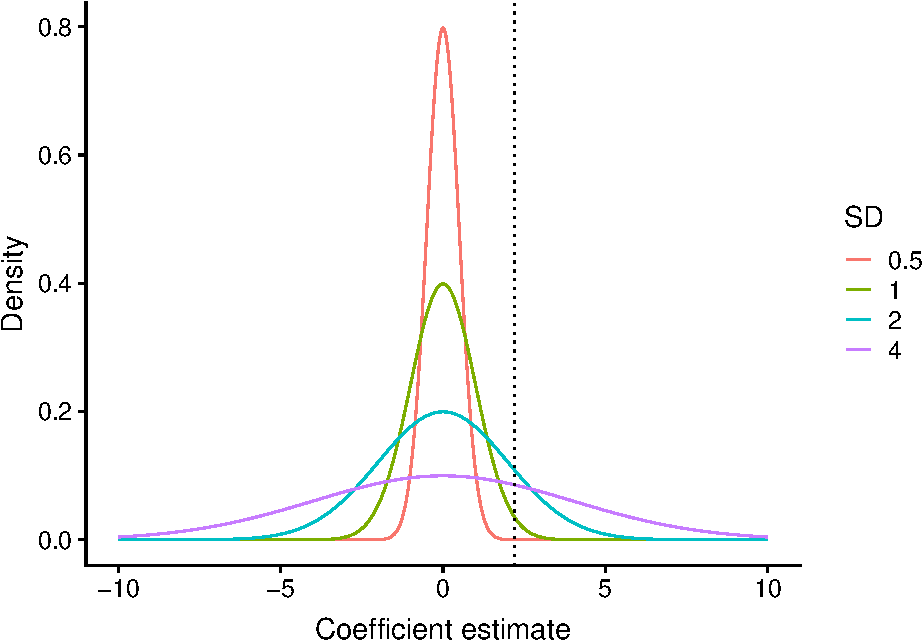
\includegraphics{reproduce_analyses_files/figure-latex/simulate prior distribution for type-1.pdf}
\caption{Simulating prior distributions for the effect of interaction
type.}
\end{figure}

Based on these distributions, we think a normal prior with mean=0 and
SD=2 would be appropriate. This creates a regularizing prior where the
mass of the distribution is centered on zero (i.e., no effect), but
allows for the model to detect large effects if the data supports it.

\subsubsection{\texorpdfstring{Subtype of interaction:
\textbf{subtype\_Herb.vs.Para} and
\textbf{subtype\_Poll.vs.Disp}}{Subtype of interaction: subtype\_Herb.vs.Para and subtype\_Poll.vs.Disp}}\label{subtype-of-interaction-subtype_herb.vs.para-and-subtype_poll.vs.disp}

We expect similar effects for different subtypes of interaction as we
would for different interaction types. Therefore, we choose to use the
same prior: normal(mean=0, SD=2).

\subsubsection{\texorpdfstring{Scaled normalized degree:
\textbf{sc.r\_ND} and
\textbf{sc.c\_ND}}{Scaled normalized degree: sc.r\_ND and sc.c\_ND}}\label{scaled-normalized-degree-sc.r_nd-and-sc.c_nd}

Since the normalized degree of a species defines its probability of
interacting with a co-occuring partner, regardless of its identity, our
prior expectation is that there is a 1:1 relationship between the
normalized degree of a species and its probability of interacting with
another species. In other words, the probability of observing an
interaction is the same as the normalized degree.

Let's get some intuition as to what this prior looks like when
normalized degree is on a standardized scale (1 SD above the mean) and
the response is in terms of log odds, which matches the assumptions of
our model. Note that we chose to only look 1 SD above the mean because
this reflects how the coefficient is estimated in the model (effect of 1
unit increase in predictor variable). We do this first for resources:

\begin{Shaded}
\begin{Highlighting}[]
\CommentTok{# probability of average species interacting}
\NormalTok{pMean_r <-}\StringTok{ }\KeywordTok{mean}\NormalTok{(full.df}\OperatorTok{$}\NormalTok{r_ND) }

\CommentTok{# probability of a relatively generalized species interacting}
\NormalTok{pGen_r <-}\StringTok{ }\KeywordTok{mean}\NormalTok{(full.df}\OperatorTok{$}\NormalTok{r_ND) }\OperatorTok{+}\StringTok{ }\KeywordTok{sd}\NormalTok{(full.df}\OperatorTok{$}\NormalTok{r_ND) }

\CommentTok{# logistic regression coefficient, which is the difference in log-odds }
\CommentTok{# for a 1 SD unit increase in a species normalized degree.}
\NormalTok{(mu_sc.r_ND <-}\StringTok{ }\KeywordTok{log}\NormalTok{(pGen_r }\OperatorTok{/}\StringTok{ }\NormalTok{(}\DecValTok{1}\OperatorTok{-}\NormalTok{pGen_r)) }\OperatorTok{-}\StringTok{ }\KeywordTok{log}\NormalTok{(pMean_r }\OperatorTok{/}\StringTok{ }\NormalTok{(}\DecValTok{1}\OperatorTok{-}\NormalTok{pMean_r))) }
\end{Highlighting}
\end{Shaded}

\begin{verbatim}
## [1] 1.040268
\end{verbatim}

and then for consumers:

\begin{Shaded}
\begin{Highlighting}[]
\NormalTok{## Consumer species }

\CommentTok{# probability of average species interacting}
\NormalTok{pMean_c <-}\StringTok{ }\KeywordTok{mean}\NormalTok{(full.df}\OperatorTok{$}\NormalTok{c_ND) }

\CommentTok{# probability of a relatively generalized species interacting}
\NormalTok{pGen_c <-}\StringTok{ }\KeywordTok{mean}\NormalTok{(full.df}\OperatorTok{$}\NormalTok{c_ND) }\OperatorTok{+}\StringTok{ }\KeywordTok{sd}\NormalTok{(full.df}\OperatorTok{$}\NormalTok{c_ND) }

\CommentTok{# logistic regression coefficient, which is the difference in log-odds }
\CommentTok{# for a 1 SD increase in a species normalized degree.}
\NormalTok{(mu_sc.c_ND <-}\StringTok{ }\KeywordTok{log}\NormalTok{(pGen_c }\OperatorTok{/}\StringTok{ }\NormalTok{(}\DecValTok{1}\OperatorTok{-}\NormalTok{pGen_c)) }\OperatorTok{-}\StringTok{ }\KeywordTok{log}\NormalTok{(pMean_c }\OperatorTok{/}\StringTok{ }\NormalTok{(}\DecValTok{1}\OperatorTok{-}\NormalTok{pMean_c))) }
\end{Highlighting}
\end{Shaded}

\begin{verbatim}
## [1] 0.9944917
\end{verbatim}

~

These examples indicate that we should have a prior expectation for the
mean estimate of these coefficients to be \textasciitilde{}1. How much
variance around this coefficient might we expect though? Let's simulate
a normal distribution with mean=1 (dotted line below), but different
variances:

\begin{figure}
\centering
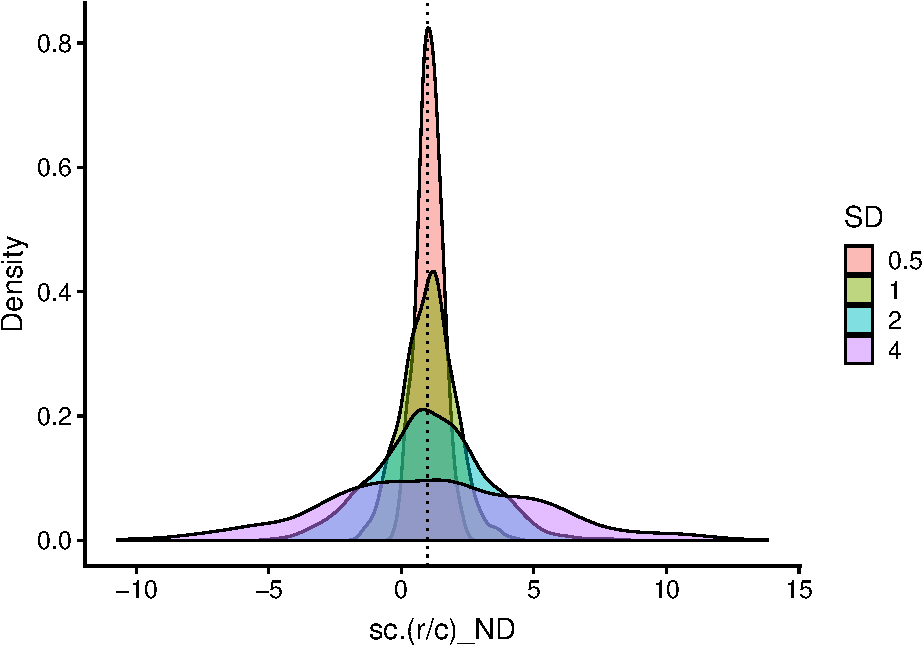
\includegraphics{reproduce_analyses_files/figure-latex/simulate prior distribution for normalized degree-1.pdf}
\caption{Simulating prior distributions for the effect of scaled
normalized degree.}
\end{figure}

Most standardized logistic regression coefficients are less than 5
\citep{Gelman2008}, so we feel that specifying a standard deviation of 2
is reasonable since it more than covers the range from 0 to 5. It will
also make the data ``work'' for larger values, since the mass of the
distribution is centered on 1.

\subsubsection{\texorpdfstring{Statistical interactions between
interaction type and normalized degree: \textbf{type\_M.vs.A:sc.r\_ND},
\textbf{type\_M.vs.A:sc.c\_ND}}{Statistical interactions between interaction type and normalized degree: type\_M.vs.A:sc.r\_ND, type\_M.vs.A:sc.c\_ND}}\label{statistical-interactions-between-interaction-type-and-normalized-degree-type_m.vs.asc.r_nd-type_m.vs.asc.c_nd}

We specified the same regularizing prior as for \textbf{type\_M.vs.A}
(i.e., normal(mean=0, SD=2)), because we have no strong prior
expectation for whether interaction type will have a positive or
negative effect on these relationships, and we want to make the data
``work'' for any strong effects.

\hypertarget{asymmetry-effect}{\subsubsection{Partner (a)symmetry
effect: sc.r\_ND:sc.c\_ND}\label{asymmetry-effect}}

Although it is not intuitive, the sign of the statistical interaction
between consumer and resource normalized degree indicates whether
partner symmetry or asymmetry increases partner fidelity. To illustrate
this, let's first assume that the main effects of scaled normalized
degree for both resources and consumers equals 1 (also our prior
expectation). For simplicity, let's assume that the statistical
interaction is either -1 or +1. With these coefficients, we can now
calculate how a change in scaled normalized degree for both resources
and consumers affects the log-odds of an interaction. Below, we explore
these effects \(\pm\) 1 SD for the scaled normalized degree of both
resources and consumers.

\begin{Shaded}
\begin{Highlighting}[]
\NormalTok{sim.log.odds <-}\StringTok{ }\KeywordTok{expand.grid}\NormalTok{(}
  \DataTypeTok{b_sc.r_ND =} \DecValTok{1}\NormalTok{, }
  \DataTypeTok{b_sc.c_ND =} \DecValTok{1}\NormalTok{,}
  \StringTok{`}\DataTypeTok{b_sc.r_ND:sc.c_ND}\StringTok{`}\NormalTok{ =}\StringTok{ }\KeywordTok{c}\NormalTok{(}\OperatorTok{-}\DecValTok{1}\NormalTok{, }\DecValTok{1}\NormalTok{),}
  \DataTypeTok{delta.sc.r_ND =} \KeywordTok{seq}\NormalTok{(}\OperatorTok{-}\DecValTok{1}\NormalTok{, }\DecValTok{1}\NormalTok{, }\FloatTok{0.01}\NormalTok{),}
  \DataTypeTok{delta.sc.c_ND =} \KeywordTok{seq}\NormalTok{(}\OperatorTok{-}\DecValTok{1}\NormalTok{, }\DecValTok{1}\NormalTok{, }\FloatTok{0.01}\NormalTok{)) }\OperatorTok
\StringTok{  }\KeywordTok{mutate}\NormalTok{(}\DataTypeTok{log.odds.connected =} 
\NormalTok{           b_sc.r_ND }\OperatorTok{*}\StringTok{ }\NormalTok{delta.sc.r_ND }\OperatorTok{+}\StringTok{                          }\CommentTok{# main effect of sc.r_ND}
\StringTok{           }\NormalTok{b_sc.c_ND }\OperatorTok{*}\StringTok{ }\NormalTok{delta.sc.c_ND }\OperatorTok{+}\StringTok{                          }\CommentTok{# main effect of sc.c_ND}
\StringTok{           `}\DataTypeTok{b_sc.r_ND:sc.c_ND}\StringTok{`} \OperatorTok{*}\StringTok{ }\NormalTok{delta.sc.r_ND }\OperatorTok{*}\StringTok{ }\NormalTok{delta.sc.c_ND, }\CommentTok{# statistical interaction}
         \DataTypeTok{main.log.odds =}\NormalTok{ b_sc.r_ND }\OperatorTok{*}\StringTok{ }\NormalTok{delta.sc.r_ND }\OperatorTok{+}\StringTok{ }\NormalTok{b_sc.c_ND }\OperatorTok{*}\StringTok{ }\NormalTok{delta.sc.c_ND,}
         \DataTypeTok{diff.log.odds =}\NormalTok{ log.odds.connected }\OperatorTok{-}\StringTok{ }\NormalTok{main.log.odds)}
\end{Highlighting}
\end{Shaded}

\begin{figure}
\centering
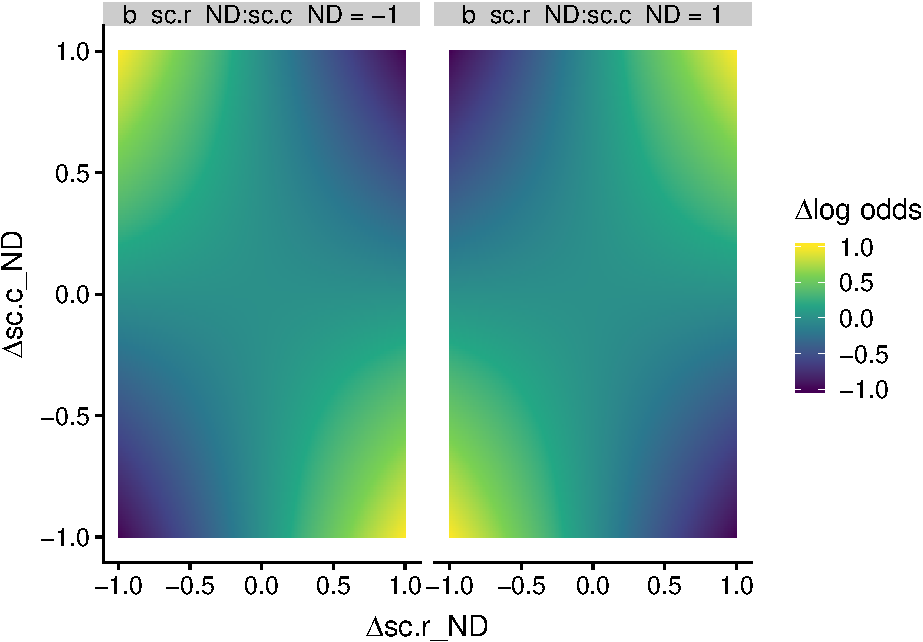
\includegraphics{reproduce_analyses_files/figure-latex/plot-NDxND-1.pdf}
\caption{\label{fig:plot-NDxND}Plot of how the sign of
b\_sc.r\_ND:sc.c\_ND determines how symmetry (righ panel) or asymmetry
(left panel) in partners normalized degree affects partner fidelity.}
\end{figure}

By inspecting figure \ref{fig:plot-NDxND}, one can see how the sign of
the statistical interaction between resource and consumer normalized
degree affects the log odds of an interaction. When the sign is positive
(right panel), symmetric normalized degrees increase the probability of
an interaction (relative to main effects). In contrast, when the sign is
negative (left panel), asymmetric normalized degrees increase the
probability of an interaction. For example, if a relatively specialized
consumer (\(\Delta\)sc.c\_ND = -1) interacts with a relatively
generalist resource (\(\Delta\)sc.r\_ND = +1), there is an increase in
the log-odds of an interaction (yellow spot in lower right corner of
left panel in fig. \ref{fig:plot-NDxND}).

Since we had no prior expectation as to how symmetry or asymmetry would
affect partner fidelity, we set a normal prior with mean=0 and SD=2 to
cover the range of most logistic regression coefficients
\citep{Gelman2008}.

\subsubsection{\texorpdfstring{Effect of mutualism on partner
(a)symmetry in normalized degrees:
\textbf{type\_M.vs.A:sc.r\_ND:sc.c\_ND}}{Effect of mutualism on partner (a)symmetry in normalized degrees: type\_M.vs.A:sc.r\_ND:sc.c\_ND}}\label{effect-of-mutualism-on-partner-asymmetry-in-normalized-degrees-type_m.vs.asc.r_ndsc.c_nd}

We again set a normal prior with mean=0 and SD=2, because we had no
strong prior expectation for how interaction type would modify the
effect of (a)symmetry in normalized degree on partner fidelity.

\subsubsection{Main effects and statistical interactions with observed
interactions
(sc.log.sum\_)}\label{main-effects-and-statistical-interactions-with-observed-interactions-sc.log.sum_}

As with normalized degree, we expect the log of observed interactions
for a resource or consumer to increase the probability of observing an
interaction between co-occuring species. Therefore, we specified the
same priors as we did for normalized degree for both main effects
(normal(mean=1, SD=2) for \textbf{sc.log.sum\_r, sc.log.sum\_c}) and
statistical interactions (normal(mean=0, SD=2) for
\textbf{sc.log.sum\_r:sc.log.sum\_c, type\_M.vs.A:sc.log.sum\_r,
type\_M.vs.A:sc.log.sum\_c, type\_M.vs.A:sc.log.sum\_r:sc.log.sum\_c}).

\subsubsection{Random effects: resource\_sp, consumer\_sp, id\_pair,
network\_id}\label{random-effects-resource_sp-consumer_sp-id_pair-network_id}

We specified a half-normal prior with mean=0 and SD=2 for each of the
random effects in our model. This prior assumes that the variance in
these effect sizes is small, but with sufficient evidence, the model can
still estimate larger effects. Note that we specify this as a normal
distribution in the code, but the R package we use constrains this prior
to only positive values since standard deviations cannot be less than
zero.

~

\subsection{Model Analyses}\label{model-analyses}

We used the \emph{brms} package \citep{Burkner2017} and its default
sampling behavior (four sampling chains for 2000 iterations each,
discarding the first 1000 iterations as burn-in) to fit these
statistical models. To mitigate bias in the posterior sampling
distribution, we set \textbf{adapt\_delta = 0.99} and
\textbf{max\_treedepth = 20}.

For the majority of our inferences below, we keep coefficients on the
log odds scale. This is because effect sizes are invariant on this
scale. For intercept terms, we make inferences on the probability scale,
and note the specific values at which this effect is measured. To
calculate probabilities, we applied the inverse logit,
\(\frac{\exp(\beta)}{\exp(\beta)+1}\), to estimates reported in each
table.

\subsubsection{Full model}\label{full-model}

\begin{Shaded}
\begin{Highlighting}[]
\NormalTok{full.brm <-}\StringTok{ }\KeywordTok{brm}\NormalTok{(}
  \DataTypeTok{formula =}\NormalTok{ interaction.formula, }\DataTypeTok{data =}\NormalTok{ full.df, }
  \DataTypeTok{prior =}\NormalTok{ interaction.priors, }\DataTypeTok{algorithm =} \StringTok{"sampling"}\NormalTok{, }
  \DataTypeTok{chains =} \DecValTok{4}\NormalTok{, }\DataTypeTok{iter =} \DecValTok{2000}\NormalTok{, }\DataTypeTok{warmup =} \DecValTok{1000}\NormalTok{, }
  \DataTypeTok{control =} \KeywordTok{list}\NormalTok{(}\DataTypeTok{adapt_delta =} \FloatTok{0.99}\NormalTok{, }\DataTypeTok{max_treedepth =} \DecValTok{20}\NormalTok{))}
\end{Highlighting}
\end{Shaded}

\begin{table}[!h]

\caption{\label{tab:full-table}Mean and 95\% credible intervals of fixed effects from our full model.}
\centering
\begin{tabular}{lrrr}
\toprule
Term & Estimate & 2.5\% & 97.5\%\\
\midrule
\rowcolor{gray!6}  Intercept & 0.63 & 0.17 & 1.05\\
type\_M.vs.A & 1.40 & 0.55 & 2.26\\
\rowcolor{gray!6}  subtype\_Herb.vs.Para & 1.30 & -0.22 & 2.75\\
subtype\_Poll.vs.Disp & 2.60 & 1.73 & 3.50\\
\rowcolor{gray!6}  sc.r\_ND & 2.00 & 1.85 & 2.16\\
sc.c\_ND & 1.51 & 1.39 & 1.64\\
\rowcolor{gray!6}  type\_M.vs.A:sc.r\_ND & 0.57 & 0.31 & 0.84\\
type\_M.vs.A:sc.c\_ND & -0.15 & -0.36 & 0.07\\
\rowcolor{gray!6}  sc.r\_ND:sc.c\_ND & 0.16 & 0.04 & 0.28\\
type\_M.vs.A:sc.r\_ND:sc.c\_ND & -0.78 & -1.01 & -0.52\\
\bottomrule
\end{tabular}
\end{table}

~

Our model provided a good fit to our data, explaining 40\% of the
variance.

\begin{Shaded}
\begin{Highlighting}[]
\KeywordTok{bayes_R2}\NormalTok{(full.brm)}
\end{Highlighting}
\end{Shaded}

\begin{verbatim}
##     Estimate   Est.Error      Q2.5     Q97.5
## R2 0.4010955 0.006517277 0.3883389 0.4139209
\end{verbatim}

~

Below, we give a biological interpretation of each term in this model
(table \ref{tab:full-table}):

\begin{itemize}
\item
  On the probability scale, the average level of partner fidelity across
  interaction types equals 0.65(\(=\frac{\exp(\beta)}{\exp(\beta)+1}\),
  where \(\beta=\) 0.63) for the average level of normalized degree for
  a resource and consumer.
\item
  Mutualistic interactions increase the log odds of partner fidelity by
  1.4 relative to antagonistic interactions.
\item
  There is no clear difference between herbivory and parasitism on
  partner fidelity (95\% credible intervals overlap with zero).
\item
  Pollination increases the log odds of partner fidelity by 2.6 relative
  to seed dispersers.
\item
  A 1 SD increase in resource normalized degree increases the log odds
  of partner fidelity by 2 across interaction types.
\item
  A 1 SD increase in consumer normalized degree increases the log odds
  of partner fidelity by 1.51 across interaction types.
\item
  Mutualistic interactions increase the positive effect of resource
  normalized degree on the log odds of partner fidelity by 0.57 relative
  to antagonistic interactions.
\item
  There is no clear evidence that mutualistic interactions (relative to
  antagonistic) modify the positive effect of consumer normalized degree
  on partner fidelity (95\% credible intervals overlap with zero).
\item
  Across interaction types, symmetry between partners in their
  normalized degree increases the log odds of partner fidelity by 0.16.
\item
  Mutualistic interactions (relative to antagonistic) decrease the
  effects of symmetry on the log odds of partner fidelity by -0.78. Put
  another way, mutualistic interactions increase the effects of
  \emph{asymmetry} on the log odds of partner fidelity by 0.78.
\end{itemize}

In addition to these fixed effects, there is considerable variation in
partner fidelity explained by our random effects. In particular,
\textbf{network\_id} has a strong effect compared to the other sources
of variation (table \ref{tab:full-table-random}).

\begin{table}[!h]

\caption{\label{tab:full-table-random}Mean and 95\% credible intervals of random effects from our full model.}
\centering
\begin{tabular}{lrrr}
\toprule
Term & Estimate & 2.5\% & 97.5\%\\
\midrule
\rowcolor{gray!6}  sd\_consumer\_sp\_\_Intercept & 0.22 & 0.12 & 0.32\\
sd\_id\_pair\_\_Intercept & 0.48 & 0.38 & 0.58\\
\rowcolor{gray!6}  sd\_network\_id\_\_Intercept & 1.47 & 1.24 & 1.74\\
sd\_resource\_sp\_\_Intercept & 0.48 & 0.37 & 0.60\\
\bottomrule
\end{tabular}
\end{table}

~

While the model above is useful for determining the effects of
mutualistic relative to antagonistic interactions on partner fidelity,
it is also useful to separately estimate relationships for mutualistic
and antagonistic interactions. We can do this by removing the intercept
term from the model, and estimating unique relationships for normalized
degree for both mutualistic and antagonistic interactions.

\begin{Shaded}
\begin{Highlighting}[]
\NormalTok{no.intercept_formula <-}\StringTok{ }\KeywordTok{brmsformula}\NormalTok{(}
\NormalTok{  connected }\OperatorTok{~}\StringTok{ }\OperatorTok{-}\DecValTok{1} \OperatorTok{+}\StringTok{ }\NormalTok{type }\OperatorTok{+}\StringTok{ }\NormalTok{subtype_Herb.vs.Para }\OperatorTok{+}\StringTok{ }\NormalTok{subtype_Poll.vs.Disp }\OperatorTok{+}\StringTok{ }
\StringTok{    }\NormalTok{type}\OperatorTok{:}\NormalTok{sc.r_ND }\OperatorTok{+}\StringTok{ }\NormalTok{type}\OperatorTok{:}\NormalTok{sc.c_ND }\OperatorTok{+}\StringTok{ }
\StringTok{    }\NormalTok{type}\OperatorTok{:}\NormalTok{sc.r_ND}\OperatorTok{:}\NormalTok{sc.c_ND }\OperatorTok{+}
\StringTok{    }\NormalTok{(}\DecValTok{1} \OperatorTok{|}\StringTok{ }\NormalTok{resource_sp) }\OperatorTok{+}\StringTok{ }\NormalTok{(}\DecValTok{1} \OperatorTok{|}\StringTok{ }\NormalTok{consumer_sp) }\OperatorTok{+}\StringTok{ }\NormalTok{(}\DecValTok{1} \OperatorTok{|}\StringTok{ }\NormalTok{id_pair) }\OperatorTok{+}\StringTok{ }\NormalTok{(}\DecValTok{1} \OperatorTok{|}\StringTok{ }\NormalTok{network_id),}
  \DataTypeTok{family =} \KeywordTok{bernoulli}\NormalTok{(}\DataTypeTok{link =} \StringTok{"logit"}\NormalTok{))}

\NormalTok{no.intercept_priors <-}\StringTok{ }\KeywordTok{c}\NormalTok{(}
  \KeywordTok{set_prior}\NormalTok{(}\StringTok{"normal(0,2)"}\NormalTok{, }\DataTypeTok{class =} \StringTok{"b"}\NormalTok{, }\DataTypeTok{coef =} \StringTok{"typeA"}\NormalTok{), }\CommentTok{# corresponds to probability of 0.5}
  \KeywordTok{set_prior}\NormalTok{(}\StringTok{"normal(0,2)"}\NormalTok{, }\DataTypeTok{class =} \StringTok{"b"}\NormalTok{, }\DataTypeTok{coef =} \StringTok{"typeM"}\NormalTok{), }\CommentTok{# corresponds to probability of 0.5}
  \KeywordTok{set_prior}\NormalTok{(}\StringTok{"normal(0,2)"}\NormalTok{, }\DataTypeTok{class =} \StringTok{"b"}\NormalTok{, }\DataTypeTok{coef =} \StringTok{"subtype_Herb.vs.Para"}\NormalTok{),}
  \KeywordTok{set_prior}\NormalTok{(}\StringTok{"normal(0,2)"}\NormalTok{, }\DataTypeTok{class =} \StringTok{"b"}\NormalTok{, }\DataTypeTok{coef =} \StringTok{"subtype_Poll.vs.Disp"}\NormalTok{),}
  \KeywordTok{set_prior}\NormalTok{(}\StringTok{"normal(1,2)"}\NormalTok{, }\DataTypeTok{class =} \StringTok{"b"}\NormalTok{, }\DataTypeTok{coef =} \StringTok{"typeA:sc.r_ND"}\NormalTok{),}
  \KeywordTok{set_prior}\NormalTok{(}\StringTok{"normal(1,2)"}\NormalTok{, }\DataTypeTok{class =} \StringTok{"b"}\NormalTok{, }\DataTypeTok{coef =} \StringTok{"typeM:sc.r_ND"}\NormalTok{),}
  \KeywordTok{set_prior}\NormalTok{(}\StringTok{"normal(1,2)"}\NormalTok{, }\DataTypeTok{class =} \StringTok{"b"}\NormalTok{, }\DataTypeTok{coef =} \StringTok{"typeA:sc.c_ND"}\NormalTok{),}
  \KeywordTok{set_prior}\NormalTok{(}\StringTok{"normal(1,2)"}\NormalTok{, }\DataTypeTok{class =} \StringTok{"b"}\NormalTok{, }\DataTypeTok{coef =} \StringTok{"typeM:sc.c_ND"}\NormalTok{),}
  \KeywordTok{set_prior}\NormalTok{(}\StringTok{"normal(0,2)"}\NormalTok{, }\DataTypeTok{class =} \StringTok{"b"}\NormalTok{, }\DataTypeTok{coef =} \StringTok{"typeA:sc.r_ND:sc.c_ND"}\NormalTok{),}
  \KeywordTok{set_prior}\NormalTok{(}\StringTok{"normal(0,2)"}\NormalTok{, }\DataTypeTok{class =} \StringTok{"b"}\NormalTok{, }\DataTypeTok{coef =} \StringTok{"typeM:sc.r_ND:sc.c_ND"}\NormalTok{),}
  \KeywordTok{set_prior}\NormalTok{(}\StringTok{"normal(0,2)"}\NormalTok{, }\DataTypeTok{class =} \StringTok{"sd"}\NormalTok{))}

\NormalTok{no.intercept_brm <-}\StringTok{ }\KeywordTok{brm}\NormalTok{(}
  \DataTypeTok{formula =}\NormalTok{ no.intercept_formula, }\DataTypeTok{data =}\NormalTok{ full.df, }
  \DataTypeTok{prior =}\NormalTok{ no.intercept_priors, }\DataTypeTok{algorithm =} \StringTok{"sampling"}\NormalTok{, }
  \DataTypeTok{chains =} \DecValTok{4}\NormalTok{, }\DataTypeTok{iter =} \DecValTok{2000}\NormalTok{, }\DataTypeTok{warmup =} \DecValTok{1000}\NormalTok{, }
  \DataTypeTok{control =} \KeywordTok{list}\NormalTok{(}\DataTypeTok{adapt_delta =} \FloatTok{0.99}\NormalTok{, }\DataTypeTok{max_treedepth =} \DecValTok{20}\NormalTok{))}
\end{Highlighting}
\end{Shaded}

~

\begin{table}[!h]

\caption{\label{tab:no-intercept-table}Mean and 95\% credible intervals of fixed effects from model without intercepts.}
\centering
\begin{tabular}{lrrr}
\toprule
Term & Estimate & 2.5\% & 97.5\%\\
\midrule
\rowcolor{gray!6}  typeA & -0.12 & -0.83 & 0.62\\
typeM & 1.35 & 0.90 & 1.78\\
\rowcolor{gray!6}  subtype\_Herb.vs.Para & 1.22 & -0.25 & 2.61\\
subtype\_Poll.vs.Disp & 2.58 & 1.65 & 3.46\\
\rowcolor{gray!6}  typeA:sc.r\_ND & 1.72 & 1.60 & 1.84\\
typeM:sc.r\_ND & 2.29 & 2.05 & 2.55\\
\rowcolor{gray!6}  typeA:sc.c\_ND & 1.59 & 1.49 & 1.70\\
typeM:sc.c\_ND & 1.44 & 1.24 & 1.64\\
\rowcolor{gray!6}  typeA:sc.r\_ND:sc.c\_ND & 0.55 & 0.43 & 0.67\\
typeM:sc.r\_ND:sc.c\_ND & -0.23 & -0.44 & -0.01\\
\bottomrule
\end{tabular}
\end{table}

~

The results from this model (table \ref{tab:no-intercept-table}) can be
interpreted as follows:

\begin{itemize}
\item
  The average level of partner fidelity for antagonistic interactions is
  0.47 (\(=\frac{\exp(\beta)}{\exp(\beta)+1}\), where \(\beta=\) -0.12)
  at the average level of normalized degree for a resource and consumer.
\item
  The average probability of partner fidelity for mutualistic
  interactions is 0.79 (\(=\frac{\exp(\beta)}{\exp(\beta)+1}\), where
  \(\beta=\) 1.35) at the average level of normalized degree for a
  resource and consumer.
\item
  A 1 SD increase in resource normalized degree in antagonistic
  interactions increases the log odds of an interaction by 1.72.
\item
  A 1 SD increase in resource normalized degree in mutualistic
  interactions increases the log odds of an interaction by 2.29.
\item
  A 1 SD increase in consumer normalized degree in antagonistic
  interactions increases the log odds of an interaction by 1.59.
\item
  A 1 SD increase in consumer normalized degree in mutualistic
  interactions increases the log odds of an interaction by 1.44.
\item
  Symmetry in partner normalized degrees increases the log odds of
  partner fidelity by 0.55 for antagonistic interactions.
\item
  Asymmetry in partner normalized degrees increases the log odds of
  partner fidelity by 0.23 for mutualistic interactions.
\end{itemize}

\subsubsection{Analysis of data subset}\label{analysis-of-data-subset}

Before testing for potential biases due to sampling effort, we test
whether we observe the same results for the data subset.

\begin{Shaded}
\begin{Highlighting}[]
\NormalTok{weighted_subset.brm <-}\StringTok{ }\KeywordTok{brm}\NormalTok{(}
  \DataTypeTok{formula =}\NormalTok{ interaction_subset.formula, }\DataTypeTok{data =}\NormalTok{ weighted_subset.df, }
  \DataTypeTok{prior =}\NormalTok{ interaction_subset.priors, }\DataTypeTok{algorithm =} \StringTok{"sampling"}\NormalTok{, }
  \DataTypeTok{chains =} \DecValTok{4}\NormalTok{, }\DataTypeTok{iter =} \DecValTok{2000}\NormalTok{, }\DataTypeTok{warmup =} \DecValTok{1000}\NormalTok{,}
  \DataTypeTok{control =} \KeywordTok{list}\NormalTok{(}\DataTypeTok{adapt_delta =} \FloatTok{0.99}\NormalTok{, }\DataTypeTok{max_treedepth =} \DecValTok{20}\NormalTok{))}
\end{Highlighting}
\end{Shaded}

\begin{table}[!h]

\caption{\label{tab:weighted-table}Mean and 95\% credible intervals of fixed effects from our weighted subset model.}
\centering
\begin{tabular}{lrrr}
\toprule
Term & Estimate & 2.5\% & 97.5\%\\
\midrule
\rowcolor{gray!6}  Intercept & 1.53 & 1.09 & 2.00\\
type\_M.vs.A & 2.85 & 2.03 & 3.70\\
\rowcolor{gray!6}  subtype\_Poll.vs.Disp & 1.57 & 0.31 & 2.81\\
sc.r\_ND & 2.04 & 1.74 & 2.35\\
\rowcolor{gray!6}  sc.c\_ND & 1.79 & 1.52 & 2.09\\
\addlinespace
type\_M.vs.A:sc.r\_ND & 0.33 & -0.21 & 0.94\\
\rowcolor{gray!6}  type\_M.vs.A:sc.c\_ND & -0.17 & -0.71 & 0.40\\
sc.r\_ND:sc.c\_ND & 0.26 & -0.02 & 0.55\\
\rowcolor{gray!6}  type\_M.vs.A:sc.r\_ND:sc.c\_ND & -0.68 & -1.22 & -0.09\\
\bottomrule
\end{tabular}
\end{table}

Note that the \textbf{Intercept} and effect of \textbf{type\_M.vs.A} is
higher in this subset of data (table \ref{tab:weighted-table}). This is
likely due to the fact that herbivory had a tendency to increase partner
fidelity (\textbf{subtype\_Herb.vs.Para} in table \ref{tab:full-table});
therefore, its absence from the data subset enhances the average
estimate of partner fidelity as well as the apparent effect of
mutualistic interactions. Other terms are similar, except that there is
less clear evidence of mutualistic interactions enhancing the effect of
resource normalized degree (\textbf{type\_M.vs.A:sc.r\_ND} in table
\ref{tab:weighted-table}), and less clear evidence of symmetry in
partner normalized degrees to positively affect partner fidelity
(\textbf{sc.r\_ND:sc.c\_ND} in table \ref{tab:weighted-table}).
Importantly, there is still clear evidence that mutualistic interactions
generally enhance partner fidelity (\textbf{type\_M.vs.A} in table
\ref{tab:weighted-table}) and also enhance the effects of
\emph{asymmetry} in partner normalized degrees on partner fidelity
(\textbf{type\_M.vs.A:sc.r\_ND:sc.c\_ND} in table
\ref{tab:weighted-table}).

As with the full model, we observe a particularly strong effect of
\textbf{network\_id} compared to the other sources of variation (table
\ref{tab:weighted-table-random}).

\begin{table}[!h]

\caption{\label{tab:weighted-table-random}Mean and 95\% credible intervals of random effects from our weighted subset model.}
\centering
\begin{tabular}{lrrr}
\toprule
Term & Estimate & 2.5\% & 97.5\%\\
\midrule
\rowcolor{gray!6}  sd\_consumer\_sp\_\_Intercept & 0.10 & 0.01 & 0.25\\
sd\_id\_pair\_\_Intercept & 0.84 & 0.72 & 0.97\\
\rowcolor{gray!6}  sd\_network\_id\_\_Intercept & 1.11 & 0.89 & 1.37\\
sd\_resource\_sp\_\_Intercept & 0.41 & 0.23 & 0.58\\
\bottomrule
\end{tabular}
\end{table}

\subsubsection{Testing for bias due to sampling
effort}\label{testing-for-bias-due-to-sampling-effort}

Our goal here is to test whether sampling effort can explain the results
we observed in the previous models, in particular, the three-way
statistical interaction with resource and consumer normalized degree. As
a reminder, we replaced normalized degree with the log of observed
interactions for both resources and consumers. The logic behind this
model is that, if we observe a three-way statistical interaction with
the observed interactions of resources and consumers, then our previous
results could simply be due to variation in sampling effort.

\begin{Shaded}
\begin{Highlighting}[]
\NormalTok{sampling_effects.brm <-}\StringTok{ }\KeywordTok{brm}\NormalTok{(}
  \DataTypeTok{formula =}\NormalTok{ sampling_effects.formula, }\DataTypeTok{data =}\NormalTok{ weighted_subset.df, }
  \DataTypeTok{prior =}\NormalTok{ sampling_effect.priors, }\DataTypeTok{algorithm =} \StringTok{"sampling"}\NormalTok{, }
  \DataTypeTok{chains =} \DecValTok{4}\NormalTok{, }\DataTypeTok{iter =} \DecValTok{2000}\NormalTok{, }\DataTypeTok{warmup =} \DecValTok{1000}\NormalTok{,}
  \DataTypeTok{control =} \KeywordTok{list}\NormalTok{(}\DataTypeTok{adapt_delta =} \FloatTok{0.99}\NormalTok{, }\DataTypeTok{max_treedepth =} \DecValTok{20}\NormalTok{))}
\end{Highlighting}
\end{Shaded}

~

\begin{table}[!h]

\caption{\label{tab:sampling-table}Mean and 95\% credible intervals of fixed effects from our sampling effects model.}
\centering
\begin{tabular}{lrrr}
\toprule
Term & Estimate & 2.5\% & 97.5\%\\
\midrule
\rowcolor{gray!6}  Intercept & 1.75 & 1.44 & 2.09\\
type\_M.vs.A & 2.89 & 2.27 & 3.52\\
\rowcolor{gray!6}  subtype\_Poll.vs.Disp & -1.06 & -1.91 & -0.18\\
sc.log.sum\_r & 1.50 & 1.31 & 1.69\\
\rowcolor{gray!6}  sc.log.sum\_c & 1.36 & 1.20 & 1.53\\
\addlinespace
type\_M.vs.A:sc.log.sum\_r & 0.72 & 0.37 & 1.09\\
\rowcolor{gray!6}  type\_M.vs.A:sc.log.sum\_c & 0.66 & 0.33 & 1.00\\
sc.log.sum\_r:sc.log.sum\_c & 0.26 & 0.10 & 0.42\\
\rowcolor{gray!6}  type\_M.vs.A:sc.log.sum\_r:sc.log.sum\_c & -0.08 & -0.39 & 0.24\\
\bottomrule
\end{tabular}
\end{table}

Inspecting the table of fixed effects (table \ref{tab:sampling-table}),
there are a few results worth noting. First, the effect of pollination
(relative to seed dispersal) on partner fidelity has reversed; in other
words, it now has a negative effect (\textbf{subtype\_Poll.vs.Disp} in
table \ref{tab:sampling-table}). Second, mutualistic interactions
increase the positive effect of observed consumer interactions on
partner fidelity (\textbf{type\_M.vs.A:sc.log.sum\_c} in table
\ref{tab:sampling-table}). Third, we do not see evidence of a three-way
interaction between the observed interactions of resources and consumers
and interaction type (\textbf{type\_M.vs.A:sc.log.sum\_r:sc.log.sum\_c}
in table \ref{tab:sampling-table}). This indicates that sampling effects
cannot explain the effect of mutualistic interactions on partner
fidelity (\textbf{type\_M.vs.A} in tables \ref{tab:full-table},
\ref{tab:weighted-table}) or the three-way interaction between
normalized degree of resources and consumers and interaction type that
we observed in previous models (\textbf{type\_M.vs.A:sc.r\_ND:sc.c\_ND}
in tables \ref{tab:full-table}, \ref{tab:weighted-table}).

The results for the random effects are similar to the other models
(tables \ref{tab:full-table-random}, \ref{tab:weighted-table-random}),
except that the most important random effect has changed to
\textbf{id\_pair}, although \textbf{network\_id} is a close second
(table \ref{tab:sampling-table-random}).

\begin{table}[!h]

\caption{\label{tab:sampling-table-random}Mean and 95\% credible intervals of random effects from our sampling effects model.}
\centering
\begin{tabular}{lrrr}
\toprule
Term & Estimate & 2.5\% & 97.5\%\\
\midrule
\rowcolor{gray!6}  sd\_consumer\_sp\_\_Intercept & 0.31 & 0.17 & 0.47\\
sd\_id\_pair\_\_Intercept & 0.71 & 0.60 & 0.82\\
\rowcolor{gray!6}  sd\_network\_id\_\_Intercept & 0.66 & 0.52 & 0.83\\
sd\_resource\_sp\_\_Intercept & 0.40 & 0.25 & 0.57\\
\bottomrule
\end{tabular}
\end{table}

\subsubsection{Alternative models to account for sampling
effort}\label{alternative-models-to-account-for-sampling-effort}

In addition to accounting for sampling effort by replacing the
normalized degree of the resource and consumer with observed
interactions, there are other ways we can account for sampling effort.
First, we could fit a model where resource and consumer observed
interactions are simply covariates in a model that includes main effects
and statistical interactions for resource and consumer normalized
degree:

\begin{Shaded}
\begin{Highlighting}[]
\NormalTok{subset.sampling_formula <-}\StringTok{ }\KeywordTok{brmsformula}\NormalTok{(}
\NormalTok{  connected }\OperatorTok{~}\StringTok{ }\NormalTok{sc.log.sum_r }\OperatorTok{+}\StringTok{ }\NormalTok{sc.log.sum_c }\OperatorTok{+}\StringTok{ }\CommentTok{# add covariates}
\StringTok{    }\NormalTok{type }\OperatorTok{+}\StringTok{ }\NormalTok{subtype_Poll.vs.Disp }\OperatorTok{+}\StringTok{ }\NormalTok{sc.r_ND }\OperatorTok{+}\StringTok{ }\NormalTok{sc.c_ND }\OperatorTok{+}
\StringTok{    }\NormalTok{type}\OperatorTok{:}\NormalTok{sc.r_ND }\OperatorTok{+}\StringTok{ }\NormalTok{type}\OperatorTok{:}\NormalTok{sc.c_ND }\OperatorTok{+}\StringTok{ }\NormalTok{sc.r_ND}\OperatorTok{:}\NormalTok{sc.c_ND }\OperatorTok{+}
\StringTok{    }\NormalTok{type}\OperatorTok{:}\NormalTok{sc.r_ND}\OperatorTok{:}\NormalTok{sc.c_ND }\OperatorTok{+}
\StringTok{    }\NormalTok{(}\DecValTok{1} \OperatorTok{|}\StringTok{ }\NormalTok{resource_sp) }\OperatorTok{+}\StringTok{ }\NormalTok{(}\DecValTok{1} \OperatorTok{|}\StringTok{ }\NormalTok{consumer_sp) }\OperatorTok{+}\StringTok{ }\NormalTok{(}\DecValTok{1} \OperatorTok{|}\StringTok{ }\NormalTok{id_pair) }\OperatorTok{+}\StringTok{ }\NormalTok{(}\DecValTok{1} \OperatorTok{|}\StringTok{ }\NormalTok{network_id),}
  \DataTypeTok{family =} \KeywordTok{bernoulli}\NormalTok{(}\DataTypeTok{link =} \StringTok{"logit"}\NormalTok{))}

\NormalTok{subset.sampling_priors <-}\StringTok{ }\KeywordTok{c}\NormalTok{(}
  \KeywordTok{set_prior}\NormalTok{(}\StringTok{"normal(1,2)"}\NormalTok{, }\DataTypeTok{class =} \StringTok{"b"}\NormalTok{, }\DataTypeTok{coef =} \StringTok{"sc.log.sum_r"}\NormalTok{),}
  \KeywordTok{set_prior}\NormalTok{(}\StringTok{"normal(1,2)"}\NormalTok{, }\DataTypeTok{class =} \StringTok{"b"}\NormalTok{, }\DataTypeTok{coef =} \StringTok{"sc.log.sum_c"}\NormalTok{),}
  \KeywordTok{set_prior}\NormalTok{(}\StringTok{"normal(0,2)"}\NormalTok{, }\DataTypeTok{class =} \StringTok{"b"}\NormalTok{, }\DataTypeTok{coef =} \StringTok{"type_M.vs.A"}\NormalTok{),}
  \KeywordTok{set_prior}\NormalTok{(}\StringTok{"normal(0,2)"}\NormalTok{, }\DataTypeTok{class =} \StringTok{"b"}\NormalTok{, }\DataTypeTok{coef =} \StringTok{"subtype_Poll.vs.Disp"}\NormalTok{),}
  \KeywordTok{set_prior}\NormalTok{(}\StringTok{"normal(1,2)"}\NormalTok{, }\DataTypeTok{class =} \StringTok{"b"}\NormalTok{, }\DataTypeTok{coef =} \StringTok{"sc.r_ND"}\NormalTok{),}
  \KeywordTok{set_prior}\NormalTok{(}\StringTok{"normal(1,2)"}\NormalTok{, }\DataTypeTok{class =} \StringTok{"b"}\NormalTok{, }\DataTypeTok{coef =} \StringTok{"sc.c_ND"}\NormalTok{),}
  \KeywordTok{set_prior}\NormalTok{(}\StringTok{"normal(0,2)"}\NormalTok{, }\DataTypeTok{class =} \StringTok{"b"}\NormalTok{, }\DataTypeTok{coef =} \StringTok{"sc.r_ND:sc.c_ND"}\NormalTok{),}
  \KeywordTok{set_prior}\NormalTok{(}\StringTok{"normal(0,2)"}\NormalTok{, }\DataTypeTok{class =} \StringTok{"b"}\NormalTok{, }\DataTypeTok{coef =} \StringTok{"type_M.vs.A:sc.r_ND"}\NormalTok{),}
  \KeywordTok{set_prior}\NormalTok{(}\StringTok{"normal(0,2)"}\NormalTok{, }\DataTypeTok{class =} \StringTok{"b"}\NormalTok{, }\DataTypeTok{coef =} \StringTok{"type_M.vs.A:sc.c_ND"}\NormalTok{),}
  \KeywordTok{set_prior}\NormalTok{(}\StringTok{"normal(0,2)"}\NormalTok{, }\DataTypeTok{class =} \StringTok{"b"}\NormalTok{, }\DataTypeTok{coef =} \StringTok{"type_M.vs.A:sc.r_ND:sc.c_ND"}\NormalTok{),}
  \KeywordTok{set_prior}\NormalTok{(}\StringTok{"normal(0,2)"}\NormalTok{, }\DataTypeTok{class =} \StringTok{"sd"}\NormalTok{))}

\NormalTok{subset.sampling_brm <-}\StringTok{ }\KeywordTok{brm}\NormalTok{(}
  \DataTypeTok{formula =}\NormalTok{ subset.sampling_formula, }\DataTypeTok{data =}\NormalTok{ weighted_subset.df, }
  \DataTypeTok{prior =}\NormalTok{ subset.sampling_priors, }\DataTypeTok{algorithm =} \StringTok{"sampling"}\NormalTok{, }
  \DataTypeTok{chains =} \DecValTok{4}\NormalTok{, }\DataTypeTok{iter =} \DecValTok{2000}\NormalTok{, }\DataTypeTok{warmup =} \DecValTok{1000}\NormalTok{, }
  \DataTypeTok{control =} \KeywordTok{list}\NormalTok{(}\DataTypeTok{adapt_delta =} \FloatTok{0.99}\NormalTok{, }\DataTypeTok{max_treedepth =} \DecValTok{20}\NormalTok{))}
\end{Highlighting}
\end{Shaded}

\begin{table}[!h]

\caption{\label{tab:subset-sampling-table}Mean and 95\% credible intervals of fixed effects from model with main effects for sampling effort.}
\centering
\begin{tabular}{lrrr}
\toprule
Term & Estimate & 2.5\% & 97.5\%\\
\midrule
\rowcolor{gray!6}  Intercept & 1.54 & 1.16 & 1.95\\
sc.log.sum\_r & 0.52 & 0.38 & 0.68\\
\rowcolor{gray!6}  sc.log.sum\_c & 0.19 & 0.07 & 0.32\\
type\_M.vs.A & 2.94 & 2.19 & 3.72\\
\rowcolor{gray!6}  subtype\_Poll.vs.Disp & 0.96 & -0.07 & 2.04\\
sc.r\_ND & 1.51 & 1.19 & 1.86\\
\rowcolor{gray!6}  sc.c\_ND & 1.62 & 1.33 & 1.92\\
type\_M.vs.A:sc.r\_ND & 0.26 & -0.29 & 0.82\\
\rowcolor{gray!6}  type\_M.vs.A:sc.c\_ND & -0.19 & -0.71 & 0.35\\
sc.r\_ND:sc.c\_ND & 0.30 & 0.03 & 0.58\\
\rowcolor{gray!6}  type\_M.vs.A:sc.r\_ND:sc.c\_ND & -0.56 & -1.10 & 0.00\\
\bottomrule
\end{tabular}
\end{table}

~

Second, we can include an additional term that accounts for (a)symmetric
effects of observed interactions (i.e.,
\textbf{sc.log.sum\_r:sc.log.sum\_c}):

\begin{Shaded}
\begin{Highlighting}[]
\NormalTok{subset.sampling.v2_formula <-}\StringTok{ }\KeywordTok{brmsformula}\NormalTok{(}
\NormalTok{  connected }\OperatorTok{~}\StringTok{ }\NormalTok{sc.log.sum_r }\OperatorTok{+}\StringTok{ }\NormalTok{sc.log.sum_c }\OperatorTok{+}\StringTok{ }\NormalTok{sc.log.sum_r}\OperatorTok{:}\NormalTok{sc.log.sum_c }\OperatorTok{+}
\StringTok{    }\NormalTok{type }\OperatorTok{+}\StringTok{ }\NormalTok{subtype_Poll.vs.Disp }\OperatorTok{+}\StringTok{ }\NormalTok{sc.r_ND }\OperatorTok{+}\StringTok{ }\NormalTok{sc.c_ND }\OperatorTok{+}
\StringTok{    }\NormalTok{type}\OperatorTok{:}\NormalTok{sc.r_ND }\OperatorTok{+}\StringTok{ }\NormalTok{type}\OperatorTok{:}\NormalTok{sc.c_ND }\OperatorTok{+}\StringTok{ }\NormalTok{sc.r_ND}\OperatorTok{:}\NormalTok{sc.c_ND }\OperatorTok{+}
\StringTok{    }\NormalTok{type}\OperatorTok{:}\NormalTok{sc.r_ND}\OperatorTok{:}\NormalTok{sc.c_ND }\OperatorTok{+}
\StringTok{    }\NormalTok{(}\DecValTok{1} \OperatorTok{|}\StringTok{ }\NormalTok{resource_sp) }\OperatorTok{+}\StringTok{ }\NormalTok{(}\DecValTok{1} \OperatorTok{|}\StringTok{ }\NormalTok{consumer_sp) }\OperatorTok{+}\StringTok{ }\NormalTok{(}\DecValTok{1} \OperatorTok{|}\StringTok{ }\NormalTok{id_pair) }\OperatorTok{+}\StringTok{ }\NormalTok{(}\DecValTok{1} \OperatorTok{|}\StringTok{ }\NormalTok{network_id),}
  \DataTypeTok{family =} \KeywordTok{bernoulli}\NormalTok{(}\DataTypeTok{link =} \StringTok{"logit"}\NormalTok{))}

\NormalTok{subset.sampling.v2_priors <-}\StringTok{ }\KeywordTok{c}\NormalTok{(}
  \KeywordTok{set_prior}\NormalTok{(}\StringTok{"normal(1,2)"}\NormalTok{, }\DataTypeTok{class =} \StringTok{"b"}\NormalTok{, }\DataTypeTok{coef =} \StringTok{"sc.log.sum_r"}\NormalTok{),}
  \KeywordTok{set_prior}\NormalTok{(}\StringTok{"normal(1,2)"}\NormalTok{, }\DataTypeTok{class =} \StringTok{"b"}\NormalTok{, }\DataTypeTok{coef =} \StringTok{"sc.log.sum_c"}\NormalTok{),}
  \KeywordTok{set_prior}\NormalTok{(}\StringTok{"normal(0,2)"}\NormalTok{, }\DataTypeTok{class =} \StringTok{"b"}\NormalTok{, }\DataTypeTok{coef =} \StringTok{"sc.log.sum_r:sc.log.sum_c"}\NormalTok{),}
  \KeywordTok{set_prior}\NormalTok{(}\StringTok{"normal(0,2)"}\NormalTok{, }\DataTypeTok{class =} \StringTok{"b"}\NormalTok{, }\DataTypeTok{coef =} \StringTok{"type_M.vs.A"}\NormalTok{),}
  \KeywordTok{set_prior}\NormalTok{(}\StringTok{"normal(0,2)"}\NormalTok{, }\DataTypeTok{class =} \StringTok{"b"}\NormalTok{, }\DataTypeTok{coef =} \StringTok{"subtype_Poll.vs.Disp"}\NormalTok{),}
  \KeywordTok{set_prior}\NormalTok{(}\StringTok{"normal(1,2)"}\NormalTok{, }\DataTypeTok{class =} \StringTok{"b"}\NormalTok{, }\DataTypeTok{coef =} \StringTok{"sc.r_ND"}\NormalTok{),}
  \KeywordTok{set_prior}\NormalTok{(}\StringTok{"normal(1,2)"}\NormalTok{, }\DataTypeTok{class =} \StringTok{"b"}\NormalTok{, }\DataTypeTok{coef =} \StringTok{"sc.c_ND"}\NormalTok{),}
  \KeywordTok{set_prior}\NormalTok{(}\StringTok{"normal(0,2)"}\NormalTok{, }\DataTypeTok{class =} \StringTok{"b"}\NormalTok{, }\DataTypeTok{coef =} \StringTok{"sc.r_ND:sc.c_ND"}\NormalTok{),}
  \KeywordTok{set_prior}\NormalTok{(}\StringTok{"normal(0,2)"}\NormalTok{, }\DataTypeTok{class =} \StringTok{"b"}\NormalTok{, }\DataTypeTok{coef =} \StringTok{"type_M.vs.A:sc.r_ND"}\NormalTok{),}
  \KeywordTok{set_prior}\NormalTok{(}\StringTok{"normal(0,2)"}\NormalTok{, }\DataTypeTok{class =} \StringTok{"b"}\NormalTok{, }\DataTypeTok{coef =} \StringTok{"type_M.vs.A:sc.c_ND"}\NormalTok{),}
  \KeywordTok{set_prior}\NormalTok{(}\StringTok{"normal(0,2)"}\NormalTok{, }\DataTypeTok{class =} \StringTok{"b"}\NormalTok{, }\DataTypeTok{coef =} \StringTok{"type_M.vs.A:sc.r_ND:sc.c_ND"}\NormalTok{),}
  \KeywordTok{set_prior}\NormalTok{(}\StringTok{"normal(0,2)"}\NormalTok{, }\DataTypeTok{class =} \StringTok{"sd"}\NormalTok{))}

\NormalTok{subset.sampling.v2_brm <-}\StringTok{ }\KeywordTok{brm}\NormalTok{(}
  \DataTypeTok{formula =}\NormalTok{ subset.sampling.v2_formula, }\DataTypeTok{data =}\NormalTok{ weighted_subset.df, }
  \DataTypeTok{prior =}\NormalTok{ subset.sampling.v2_priors, }\DataTypeTok{algorithm =} \StringTok{"sampling"}\NormalTok{, }
  \DataTypeTok{chains =} \DecValTok{4}\NormalTok{, }\DataTypeTok{iter =} \DecValTok{2000}\NormalTok{, }\DataTypeTok{warmup =} \DecValTok{1000}\NormalTok{, }
  \DataTypeTok{control =} \KeywordTok{list}\NormalTok{(}\DataTypeTok{adapt_delta =} \FloatTok{0.99}\NormalTok{, }\DataTypeTok{max_treedepth =} \DecValTok{20}\NormalTok{))}
\end{Highlighting}
\end{Shaded}

\begin{table}[!h]

\caption{\label{tab:subset-sampling-v2-table}Mean and 95\% credible intervals of fixed effects from model that includes covariates for observed interactions of resources and consumers and their statistical interaction.}
\centering
\begin{tabular}{lrrr}
\toprule
Term & Estimate & 2.5\% & 97.5\%\\
\midrule
\rowcolor{gray!6}  Intercept & 1.53 & 1.13 & 1.94\\
sc.log.sum\_r & 0.52 & 0.37 & 0.67\\
\rowcolor{gray!6}  sc.log.sum\_c & 0.16 & 0.03 & 0.28\\
type\_M.vs.A & 2.96 & 2.20 & 3.77\\
\rowcolor{gray!6}  subtype\_Poll.vs.Disp & 1.22 & 0.19 & 2.28\\
sc.r\_ND & 1.53 & 1.21 & 1.86\\
\rowcolor{gray!6}  sc.c\_ND & 1.67 & 1.37 & 1.97\\
sc.log.sum\_r:sc.log.sum\_c & 0.21 & 0.10 & 0.31\\
\rowcolor{gray!6}  type\_M.vs.A:sc.r\_ND & 0.30 & -0.26 & 0.89\\
type\_M.vs.A:sc.c\_ND & -0.12 & -0.66 & 0.43\\
\rowcolor{gray!6}  sc.r\_ND:sc.c\_ND & 0.15 & -0.13 & 0.43\\
type\_M.vs.A:sc.r\_ND:sc.c\_ND & -0.62 & -1.16 & -0.08\\
\bottomrule
\end{tabular}
\end{table}

Inspecting table \ref{tab:subset-sampling-table} and table
\ref{tab:subset-sampling-v2-table}, we see that our key results are
robust. Specifically, mutualistic interactions generally enhance partner
fidelity and also enhance the effects of \emph{asymmetry} in partner
normalized degrees on partner fidelity.

\subsection{Robustness to Different
Priors}\label{robustness-to-different-priors}

To test how robust our results were to a different choice of priors, we
re-analyzed the full model with the default priors from the \emph{brms}
package, which are designed to be non or very weakly informative. Note
that we had to increase \textbf{adapt\_delta = 0.999} to avoid bias in
the posterior sampling of this model.

\begin{Shaded}
\begin{Highlighting}[]
\NormalTok{nopriors.brm <-}\StringTok{ }\KeywordTok{brm}\NormalTok{(}
  \DataTypeTok{formula =}\NormalTok{ interaction.formula, }\DataTypeTok{data =}\NormalTok{ full.df, }
  \CommentTok{# prior = interaction.priors, # remove and use default priors}
  \DataTypeTok{algorithm =} \StringTok{"sampling"}\NormalTok{, }\DataTypeTok{chains =} \DecValTok{4}\NormalTok{, }\DataTypeTok{iter =} \DecValTok{2000}\NormalTok{, }\DataTypeTok{warmup =} \DecValTok{1000}\NormalTok{, }
  \DataTypeTok{control =} \KeywordTok{list}\NormalTok{(}\DataTypeTok{adapt_delta =} \FloatTok{0.999}\NormalTok{, }\DataTypeTok{max_treedepth =} \DecValTok{20}\NormalTok{))}
\end{Highlighting}
\end{Shaded}

\begin{table}[!h]

\caption{\label{tab:nopriors-table}Mean and 95\% credible intervals of fixed effects from the no priors model.}
\centering
\begin{tabular}{lrrr}
\toprule
Term & Estimate & 2.5\% & 97.5\%\\
\midrule
\rowcolor{gray!6}  Intercept & 0.65 & 0.16 & 1.12\\
type\_M.vs.A & 1.40 & 0.46 & 2.29\\
\rowcolor{gray!6}  subtype\_Herb.vs.Para & 1.40 & -0.18 & 3.01\\
subtype\_Poll.vs.Disp & 2.72 & 1.83 & 3.64\\
\rowcolor{gray!6}  sc.r\_ND & 2.01 & 1.86 & 2.18\\
\addlinespace
sc.c\_ND & 1.52 & 1.41 & 1.64\\
\rowcolor{gray!6}  type\_M.vs.A:sc.r\_ND & 0.59 & 0.32 & 0.87\\
type\_M.vs.A:sc.c\_ND & -0.14 & -0.35 & 0.07\\
\rowcolor{gray!6}  sc.r\_ND:sc.c\_ND & 0.16 & 0.04 & 0.28\\
type\_M.vs.A:sc.r\_ND:sc.c\_ND & -0.78 & -1.01 & -0.52\\
\bottomrule
\end{tabular}
\end{table}

\begin{table}[!h]

\caption{\label{tab:nopriors-table-random}Mean and 95\% credible intervals of random effects from the no priors model.}
\centering
\begin{tabular}{lrrr}
\toprule
Term & Estimate & 2.5\% & 97.5\%\\
\midrule
\rowcolor{gray!6}  sd\_consumer\_sp\_\_Intercept & 0.22 & 0.12 & 0.31\\
sd\_id\_pair\_\_Intercept & 0.49 & 0.39 & 0.58\\
\rowcolor{gray!6}  sd\_network\_id\_\_Intercept & 1.49 & 1.25 & 1.76\\
sd\_resource\_sp\_\_Intercept & 0.49 & 0.38 & 0.61\\
\bottomrule
\end{tabular}
\end{table}

There is an incredibly close correspondence between these results
(tables \ref{tab:nopriors-table}, \ref{tab:nopriors-table-random}) and
the one where we specified the priors (tables \ref{tab:full-table},
\ref{tab:full-table-random}), indicating that our results are robust.

\bibliography{references}


\end{document}
